% !TeX program = lualatex
\providecommand\DocumentMetadata[1]{}
\DocumentMetadata{
  lang=en-US,
  pdfversion=2.0
}
\PassOptionsToPackage{numbers,sort&compress}{natbib}
\documentclass[proposalMode]{ufdissertation}
\sloppy

\usepackage{booktabs,array}
\usepackage{graphicx}
\usepackage{enumitem}
\usepackage{microtype}
\usepackage{bookmark}
\usepackage{xurl}
\makeatletter
% The UF class reads the main auxiliary file before bookmark activates its
% handler under LuaLaTeX.  Keep those entries inert during the early read;
% bookmark installs the real handler at \begin{document}.
\providecommand\BKM@entry[2]{}
\makeatother
% UF requires one journal to serve as the exact reference-style model.
% This proposal follows Scripta Materialia's Elsevier numbered style.
\setlength{\bibsep}{\baselineskip}

\setlist[itemize]{leftmargin=*,itemsep=0.25em}
\setlist[enumerate]{leftmargin=*,itemsep=0.25em}
\renewcommand{\arraystretch}{1.2}
\hypersetup{
  pdftitle={From Controlled Simulations to 4D Experiments: Local Machine Learning of Grain-Growth Dynamics},
  pdfauthor={Zhihui Tian},
  pdfsubject={Ph.D. Proposal}
}

\title{From Controlled Simulations to 4D Experiments: Local Machine Learning of Grain-Growth Dynamics}
\author{Zhihui Tian}
\thesisType{Ph.D. Proposal}
\degreeType{Doctor of Philosophy}
\major{Electrical and Computer Engineering}
\degreeMonth{May}
\degreeYear{2027}
\proposalDate{August 6, 2026}
\chair{Joel B. Harley}
\committeeMembers{Michael Tonks, Alina Zare, Sanjeev Koppal}

\haveTablestrue
\haveFigurestrue

\setAbstractFile{proposal_abstract}
\setReferenceFile{references}{elsarticle-num}

\begin{document}

\clearpage
\section*{Research Status and Evidence Convention}
\addcontentsline{toc}{chapter}{RESEARCH STATUS AND EVIDENCE CONVENTION}

The work described here spans three levels of research maturity, and the text labels which level every claim rests on:

\begin{itemize}

\item \textbf{Completed prior work:} the neighborhood-driven anisotropy and lattice-pinning study and 3D-PRIMME. The 3D-PRIMME manuscript is currently under review.

\item \textbf{Ongoing work with stable preliminary results:} the experimental-surrogate study, including every result reported in the current manuscript.

\item \textbf{Proposed future work:} multi-window reliability and uncertainty assessment, training-blind system validation of the experiment-trained surrogate, and interpretability and physics learning applied to reliable experiment-trained models; input- and output-side probing are the interpretation methods currently developed.

\end{itemize}

Formal citations identify the manuscript or external literature supporting each claim. Where a threshold must be fixed prospectively, before the data that would set it are examined, the placeholder \texttt{[NEEDS QUANTITATIVE CRITERION]} marks the decision as deliberately deferred.

\chapter{Introduction and Research Vision}

\section{Mesoscale prediction as a local-to-global problem}

Grain growth is expressed macroscopically through changes in grain size, size distribution, topology, and morphology, but these observables emerge from local motion and rearrangement near grain boundaries. Predictive modeling has to bridge two scales: the local neighborhood in which an interface update occurs, and the large spatial and temporal domain over which those updates accumulate into measurable microstructural evolution. Established Monte Carlo, phase-field, and geometric approaches expose complementary kinetic, topological, and three-dimensional aspects of this problem~\cite{mullins1956motion,hillert1965growth,anderson1984kinetics,srolovitz1984topology,chen2002phasefield,krill2002phasefield,macpherson2007vonneumann,lazar2011threeD}. Direct three-dimensional simulation over experimentally relevant volumes and long time horizons remains computationally demanding, motivating learned surrogates that can reproduce local updates more efficiently~\cite{montes2021surrogate,yan2022primme,qin2024graingnn,tian2026threeDprimme}.

Machine learning does not remove the need to define physical content. A supervised model learns the relationships contained in its labels. When the labels come from simulation, the learned operator is limited by the simulator's assumptions, discretization, stochastic policy, and numerical artifacts. When the labels come from experiment, the model may also learn acquisition motion, reconstruction and segmentation error, and identity-linkage failures as if they were physical boundary motion. Fitting voxel transitions is the easy part of this problem. The harder question is whether the whole path from data source to local operator to long rollout can be trusted physically and statistically.

\section{Position relative to existing approaches}

Physics-based grain-growth models and learned surrogates answer different parts of the local-to-global problem. Monte Carlo and mode-filter methods provide efficient stochastic evolution with explicit control over the local update policy; phase-field methods resolve diffuse-interface evolution from prescribed free-energy and kinetic models; and geometric or topological descriptions expose relations among boundary motion, grain size, and connectivity~\cite{anderson1984kinetics,chen2002phasefield,krill2002phasefield,macpherson2007vonneumann,melville2024modefilter}. These approaches remain essential reference models, but applying them directly to a sparse sequence of categorical experimental grain maps still requires assumptions about constitutive parameters, temporal calibration, boundary conditions, and measurement uncertainty.

Existing machine-learning approaches span phase-field-trained surrogates, local physics-regularized update models, dynamic graph models for three-dimensional microstructures, and high-fidelity deep-learning accelerators~\cite{montes2021surrogate,yan2022primme,qin2024graingnn,tep2025grain}. Their representations, supervision, and validation targets differ in concrete ways. The phase-field surrogate of Montes de Oca Zapiain \emph{et al.} evolves a global low-dimensional representation of simulated two-phase spinodal decomposition. The original PRIMME learns two-dimensional Monte-Carlo-Potts neighbor transitions, whereas GrainGNN uses phase-field-labeled, hand-crafted grain/junction graphs to predict three-dimensional epitaxial grain formation. The autoencoder--ConvLSTM model of Tep and Bernacki operates on simulator-generated two-dimensional image sequences and emphasizes image similarity, mean size, distributions, and computational acceleration. A fixed three-dimensional local operator, by comparison, decouples the learned input size from the global inference volume, turns one volume into many boundary-centered examples, and can be evaluated through categorical voxel transitions as well as kinetics, topology, morphology, and inclination response. The completed 3D-PRIMME work tests this latter hypothesis explicitly through rollout, spatial scaling, topology, and prescribed-anisotropy experiments.

This dissertation does not claim that local learning replaces phase-field, graph, or other surrogate formulations. Its contribution is a source-aware program organized around three questions: which local rule is present in the labels, whether that rule can be learned and scaled, and what additional evidence becomes necessary when the teacher changes from a controlled simulator to sparse 4D measurement. In the experimental setting, curation, grouped validation, null models, and field-level artifact diagnostics are part of the scientific method, not auxiliary preprocessing.

\section{Overarching research question}

This dissertation asks:

\begin{quote}

\textbf{How can local, physics-guided machine learning progress from learning physically controlled simulation dynamics to learning reliably from sparse 4D experimental observations, and ultimately support physical interpretation of mesoscale grain growth?}

\end{quote}

The question is addressed through a sequence of progressively removed assumptions:

\begin{enumerate}

\item diagnose how a stochastic simulation neighborhood determines the physical content and artifacts of simulation labels;

\item test whether a scalable local surrogate can learn those controlled simulation rules;

\item replace simulation labels with curated experimental evolution;

\item test the resulting operator once against experimental observations used for neither training nor model selection;

\item interpret only those experimentally learned relationships that pass the relevant reliability tests.

\end{enumerate}

\section{Central hypothesis}

The central hypothesis is:

\begin{quote}

\textbf{Local grain-growth evolution is sufficiently encoded in carefully curated neighborhood observations to support reliable three-dimensional prediction across held-out partitions of the available experimental volume; empirical uncertainty and sensitivity assessment can identify unsupported predictions, while a single training-blind validation of experiment-trained predictions against unseen experimental observations can establish which learned relationships are reliable enough for subsequent physical interpretation.}

\end{quote}

This hypothesis does not assume that agreement with a simulator proves agreement with nature, that one selected experimental window establishes generalization, or that accurate prediction automatically identifies a mechanism. Instead, it makes reliability conditional on the data source, validation level, and domain of applicability.

The hypothesis has operational failure conditions. It will not be supported if held-out error increases without a corresponding increase in the proposed warning or uncertainty score; if acceptable performance cannot be reproduced across any prespecified experimental partition; if field-level artifact diagnostics fail while aggregate metrics appear favorable; or if interpretation signatures are not reproducible across model initializations and eligible windows. The third failure mode is not hypothetical: an uncurated model produced roughly \(3.5\) voxels per step of rigid drift while its population statistics still looked favorable~\cite{tian2026experiment}.

\section{Dissertation logic and significance}

The dissertation follows the causal chain:

\begin{quote}

\textbf{Neighborhood-controlled simulation physics   \(\rightarrow\) scalable simulation-trained surrogate   \(\rightarrow\) reliable experimental learning   \(\rightarrow\) training-blind system validation   \(\rightarrow\) physical interpretation}

\end{quote}

The first two stages are completed foundations. They establish that local simulation rules can be physically diagnosed and that a compact local architecture can learn and scale those rules. The experimental study then demonstrates that the architecture can be trained directly from measured grain-ID evolution after careful curation. Changing the label generator removes the simulator from the supervision path, but this dissertation does not assume that the resulting model has thereby identified physical content absent from the simulator. The proposed work addresses what the preliminary study cannot yet establish: reliability across partitions of the available volume, a defensible uncertainty/domain-of-applicability framework, a single training-blind validation of the experiment-trained operator, and eventually a testable interpretation of experimentally learned responses.

\begin{figure}[htbp]
\centering
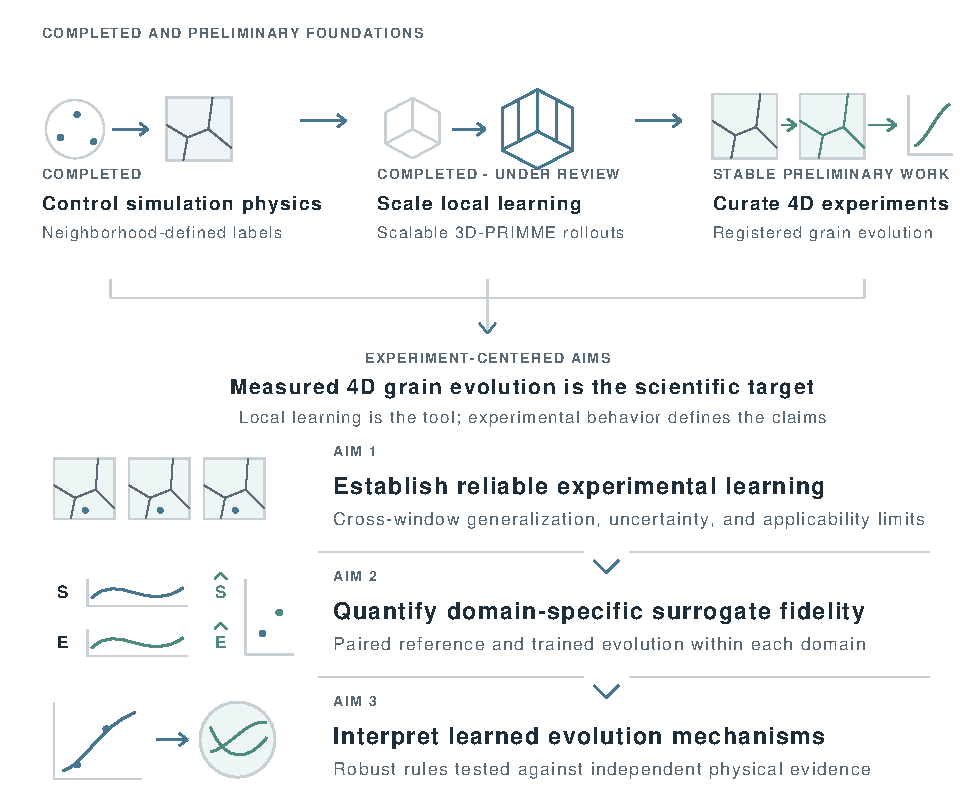
\includegraphics[alt={Research workflow from simulation foundations through three dependent experimental aims},width=0.96\textwidth]{figures/proposal_framework.pdf}
\caption{Overview of the dissertation research program. Completed simulation foundations and stable preliminary experimental work support three dependent, experiment-centered aims. Reliability is established first; a single training-blind test then adjudicates each metric family; only validated outputs advance to physical interpretation.}
\label{fig:proposal-framework}
\end{figure}

\section{Evidence ladder and claim discipline}

The dissertation uses one evidence ladder throughout (Table~\ref{tab:evidence-ladder}). Each level requires the preceding level but supports a stronger scientific statement. This hierarchy prevents label agreement, rollout fidelity, model interpretation, physical attribution, and mechanism testing from being treated as interchangeable.

\begin{table}[htbp]
\centering
\caption{Evidence ladder used to delimit the claims of the completed work and proposed aims.}
\label{tab:evidence-ladder}
\small
\begin{tabularx}{\textwidth}{@{}p{0.07\textwidth}X p{0.30\textwidth}@{}}
\toprule
\textbf{Level} & \textbf{Evidence required} & \textbf{Role in this dissertation} \\
\midrule
1 & \textbf{Label and field integrity:} registration, linkage, boundary updates, drift, and coherent-artifact checks & established in curation; extended in Aim 1 \\
2 & \textbf{Mesoscale predictive fidelity:} kinetics, distributions, topology, morphology, and grain-level response relative to the appropriate reference & established for key simulation outputs; established for experiment in Aim 1; confirmed on a training-blind experimental partition in Aim 2 \\
3 & \textbf{Stable model interpretation:} reproducible scale attribution and input--output response structure & simulation-domain methods completed; experimental transfer in Aim 3 \\
4 & \textbf{Physical attribution:} stable model responses associated with measurable physical descriptors under controls & conditional Aim 3 outcome \\
5 & \textbf{Candidate mechanism:} falsifiable prediction or intervention beyond pattern agreement & enabled but not guaranteed \\
\bottomrule
\end{tabularx}
\end{table}


\chapter{Completed Foundations: From Simulation Physics to 3D Surrogate Learning}

\textbf{Research status: COMPLETED PRIOR WORK}

\section{Neighborhood-dependent simulation physics}
\label{sec:neighborhood-physics}

\subsection{Stochastic update rules and neighborhood geometry}

Stochastic lattice and voxel models represent a microstructure through discrete grain identities and update those identities according to local rules. Their computational accessibility makes them useful for generating long sequences and large training sets, but their effective behavior depends on more than the nominal physical objective. Neighborhood shape, lattice discretization, sampling count, pseudo-temperature, update acceptance, and spatially varying mobility each leave a mark on the resulting inclination preference, pinning, morphology, topology, and grain-level statistical scatter~\cite{wu1982potts,anderson1984kinetics,srolovitz1984topology,holm1998mobility,melville2024modefilter,tian2026neighborhood}.

The conventional Monte Carlo Potts model evaluates a local Hamiltonian in a fixed neighborhood, proposes an identity change, and accepts or rejects it based on the resulting energy change and pseudo-temperature. For site \(i\), the local energy and acceptance rule are

\begin{equation}
\begin{aligned}
\mathcal{H}_i
&=
\frac{1}{2}\sum_{j\in\mathcal{N}_i}
\gamma_{ij}\left(1-\delta_{s_i,s_j}\right),\\
\Delta\mathcal{H}_i
&=
\mathcal{H}'_i-\mathcal{H}_i,\\
p(\Delta\mathcal{H}_i)
&=
\begin{cases}
\exp\!\left(-\dfrac{\Delta\mathcal{H}_i}{kT}\right),
& \Delta\mathcal{H}_i>0,\\[4pt]
1, & \Delta\mathcal{H}_i\le 0,
\end{cases}
\end{aligned}
\label{eq:mcp-update}
\end{equation}

Here, \(s_i\) is the grain identity at site \(i\), \(\mathcal{N}_i\) is its neighborhood, \(\gamma_{ij}\) is the relative boundary energy, \(T\) is the pseudo-temperature, and \(\delta\) is the Kronecker delta. The mode filter instead samples sites from a positive symmetric kernel and assigns the most frequent sampled identity. Neighborhood-driven MCP replaces the fixed Moore neighborhood with samples from an arbitrary probability mass function while retaining the MCP acceptance rule. These methods provide a controlled setting in which the influence of neighborhood geometry can be separated from other parts of the update policy~\cite{wu1982potts,anderson1984kinetics,melville2024modefilter,tian2026neighborhood}.

The neighborhood study investigates why stochastic grain-growth models develop lattice pinning and inclination-dependent artifacts. Its central contribution is to show that the local neighborhood is not a neutral numerical stencil. The first absolute moment of the sampling kernel defines an effective inclination-dependent interfacial energy, which can be connected through a Wulff construction to equilibrium shape and inclination distribution. Discrete sampling and stochastic update policy determine how sharply that theoretical response is expressed~\cite{tian2026neighborhood}.

For a continuous two-dimensional kernel \(K(x,y)\), the inclination-dependent interfacial energy and its discrete-lattice counterpart are

\begin{equation}
\begin{aligned}
\gamma(\theta)
&=
\int_{\mathbb{R}^2}
K(x,y)\,
\left|x\cos\theta+y\sin\theta\right|
\,\mathrm{d}x\,\mathrm{d}y,\\
\gamma_d(\theta)
&=
\sum_{m=1}^{M}
K(x_m,y_m)\,
\left|x_m\cos\theta+y_m\sin\theta\right|.
\end{aligned}
\label{eq:kernel-energy}
\end{equation}

Thus, neighborhood geometry enters the effective physics through a directional first absolute moment. The corresponding equilibrium Wulff shape is

\begin{equation}
W=
\bigcap_{\theta\in(0,2\pi]}
\left\{
(x,y)\in\mathbb{R}^2:
x\cos\theta+y\sin\theta\le\gamma(\theta)
\right\}.
\label{eq:wulff}
\end{equation}

Equations~\eqref{eq:kernel-energy}--\eqref{eq:wulff} make the causal chain explicit: changing \(K\) changes \(\gamma(\theta)\), which changes the preferred equilibrium shape and its boundary-inclination population.

The same directional-moment argument extends to a three-dimensional kernel. For unit interface normal \(\hat{\mathbf n}\),

\begin{equation}
\gamma(\hat{\mathbf n})
=
\int_{\mathbb{R}^3}
K(\mathbf r)
\left|\mathbf r\cdot\hat{\mathbf n}\right|
\,\mathrm{d}\mathbf r,
\qquad
W_3
=
\bigcap_{\hat{\mathbf n}\in\mathbb{S}^2}
\left\{
\mathbf x\in\mathbb{R}^3:
\mathbf x\cdot\hat{\mathbf n}\le\gamma(\hat{\mathbf n})
\right\}.
\label{eq:kernel-energy-3d}
\end{equation}

Equation~\eqref{eq:kernel-energy-3d} supplies the dimensional bridge used in the dissertation: a three-dimensional sampling distribution prescribes a directional response over interface normals rather than planar angles. A literal three-dimensional extension of a planar star kernel would inherit the symmetry of its selected arms, commonly producing axial or cubic preferences instead of rotational invariance. The downstream 3D-PRIMME study instead uses Gaussian kernels whose covariance provides a compact, controlled way to impose isotropic or \([111]\)-biased sampling.

\begin{figure}[htbp]
\centering
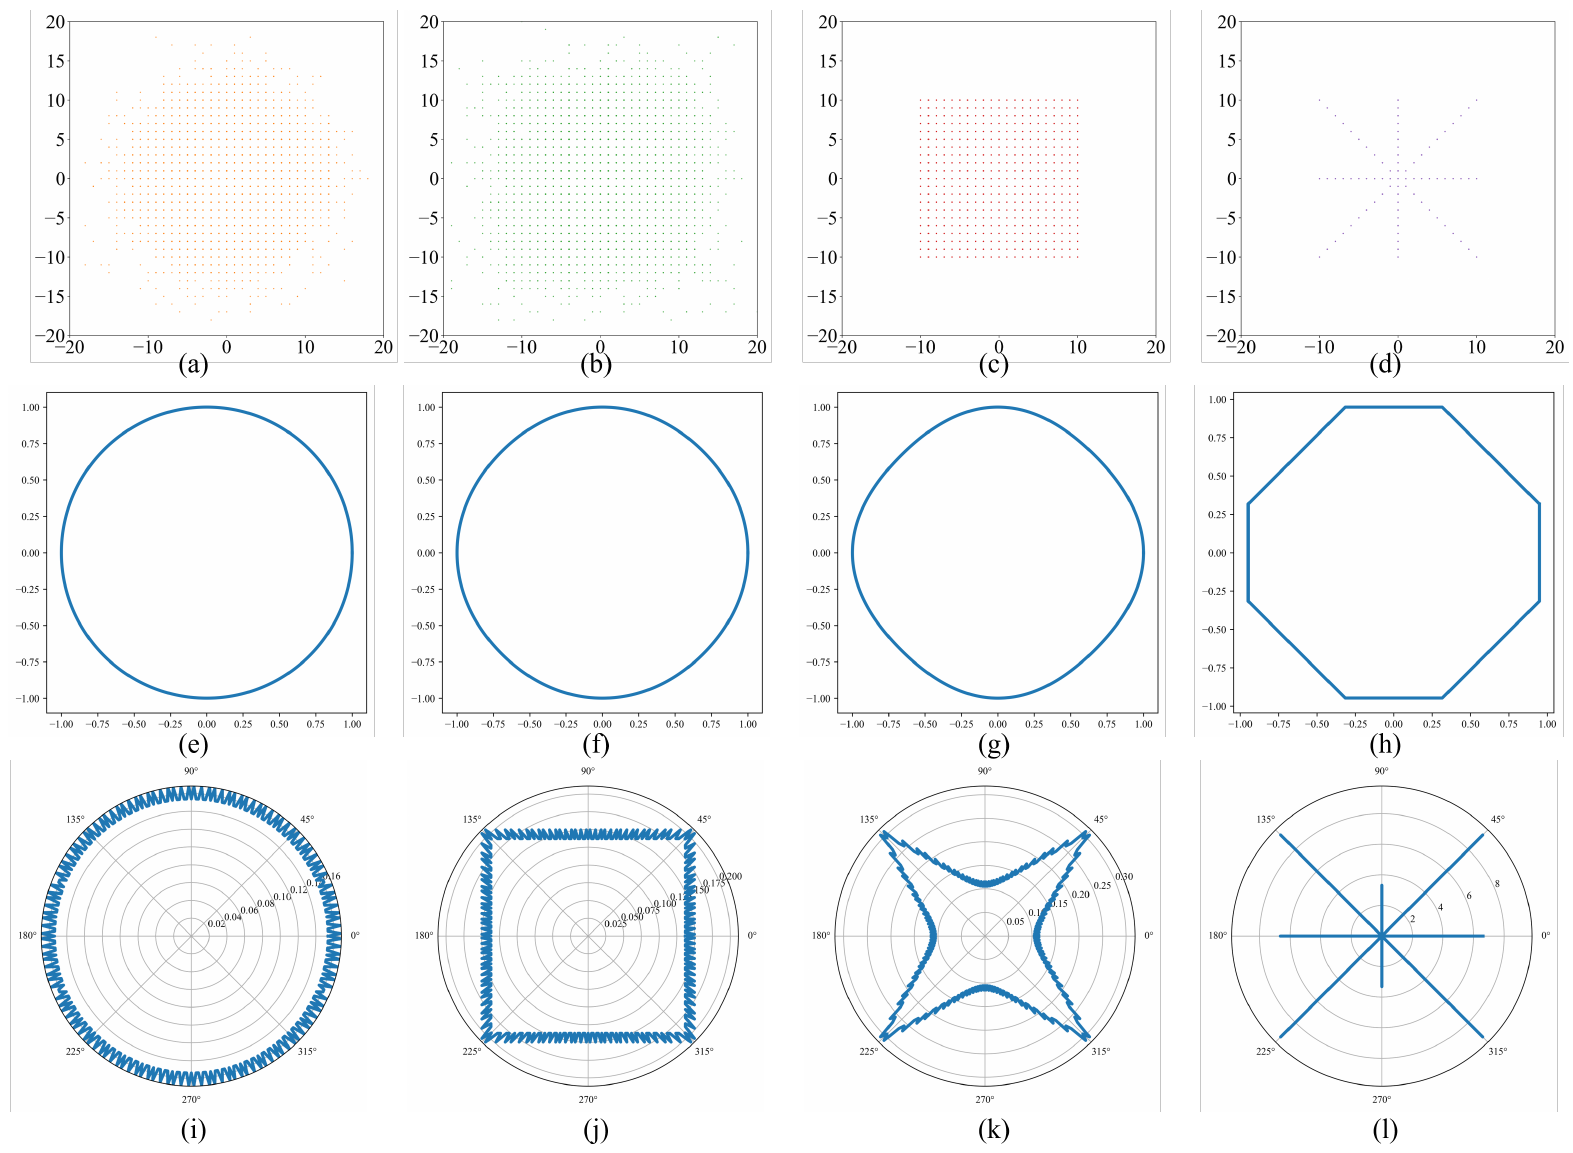
\includegraphics[alt={Sampling neighborhoods, theoretical Wulff shapes, and predicted inclination distributions},width=0.96\textwidth]{figures/neighborhood_kernel_wulff.png}
\caption{Sampling neighborhoods (top), corresponding theoretical Wulff shapes (middle), and predicted inclination distributions (bottom) for the neighborhood families evaluated in the completed study. Adapted from Fig.~1 of the Neighborhood manuscript.}
\label{fig:neighborhood-kernel-wulff}
\end{figure}

For surrogate learning, this result reframes simulator design as training-data governance. A neural operator trained on simulation does not see an abstract law; it sees updates generated by a particular kernel and update policy. Artificial directional preference in the simulator becomes an artificial directional preference available for learning. Conversely, a deliberately anisotropic neighborhood can provide controlled labels for testing whether a model recovers a prescribed response.

\subsection{Methods}

The completed study compares MCP, N-MCP, and MF evolution in \(2400\times2400\)-pixel domains initialized from a common 20,000-grain Voronoi tessellation. Comparisons are performed at matched grain counts because neighborhood choice changes the evolution rate. Gaussian, reshaped-Gaussian, square, and star-shaped sampling neighborhoods are used to vary inclination dependence systematically. The analysis evaluates theoretical and simulated inclination distributions, aggregate anisotropy magnitude, equilibrium morphology, rotation of the imposed anisotropy, von Neumann-Mullins behavior, statistical scatter, and computational cost~\cite{tian2026neighborhood}.

\subsection{Completed results}

Conventional zero-temperature MCP exhibits strong lattice-aligned boundary populations. Increasing pseudo-temperature softens this response, while N-MCP with Gaussian sampling yields an approximately circular inclination distribution in the tested conditions. Progressing from Gaussian to reshaped Gaussian, square, and star neighborhoods produces progressively stronger directional preferences. MF exhibits the same qualitative dependence: the Gaussian case is nearly isotropic, while non-circular neighborhoods generate stronger anisotropy~\cite{tian2026neighborhood}.

The rotation test provides the clearest causal evidence. Rotating reshaped-Gaussian and uniform MF neighborhoods by 0, 30, and 60 degrees rotates the measured inclination response accordingly. This separates the orientation of the neighborhood from the fixed orientation of the pixel grid. The work further shows that neighborhood geometry and algorithmic stochasticity affect different observables: MF produces substantially lower scatter in the reported von Neumann-Mullins comparison than MCP and N-MCP, while changing the N-MCP neighborhood alone does not eliminate grain-level scatter. Increasing the number of MF samples improves statistical stability~\cite{tian2026neighborhood}.

\begin{figure}[htbp]
\centering
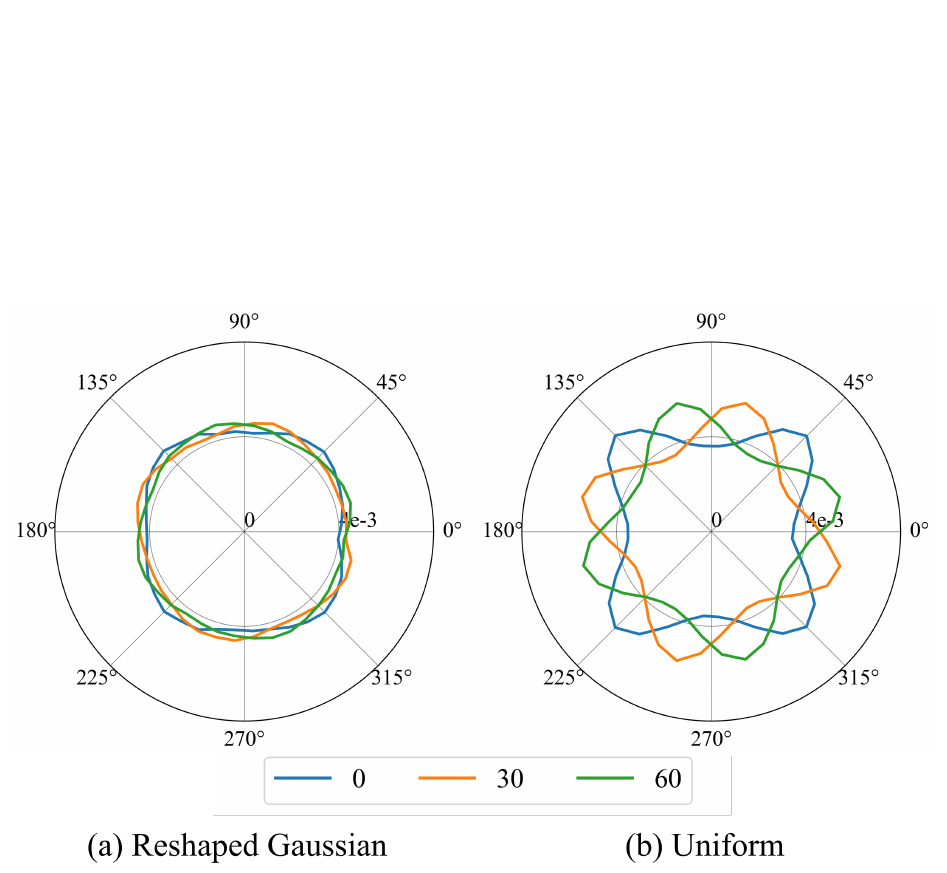
\includegraphics[alt={Inclination distributions rotating with reshaped-Gaussian and uniform mode-filter neighborhoods},width=0.68\textwidth]{figures/neighborhood_rotation_test.png}
\caption{Measured inclination distributions after rotating reshaped-Gaussian and uniform MF neighborhoods by \(0^\circ\), \(30^\circ\), and \(60^\circ\). The response rotates with the neighborhood, providing a causal separation from the fixed pixel lattice. Adapted from Fig.~6 of the Neighborhood manuscript.}
\label{fig:neighborhood-rotation}
\end{figure}

\subsection{Role and claim boundary}

This work establishes control with respect to lattice pinning, artificial inclination preference, and selected topological/statistical behavior. It does not establish correct material-specific mobility, misorientation dependence, boundary energy, or agreement with experimental alumina. The defensible dissertation claim is therefore:

\begin{quote}

The neighborhood study provides the physical basis for selecting and diagnosing the simulation teacher used for surrogate training.

\end{quote}

It should not be claimed that the study directly proved improved 3D-PRIMME accuracy, because no surrogate was trained on paired ``poor'' and ``improved'' neighborhood datasets. Its enabling role is conceptual and methodological: it identifies which local rules are present in the simulation labels and provides controlled isotropic and anisotropic teachers for the next stage.

\bigskip

\section{Simulation-trained 3D-PRIMME}

\textbf{Research status: COMPLETED PRIOR WORK; MANUSCRIPT UNDER REVIEW}

A local surrogate represents evolution through a fixed neighborhood operator instead of a global map over the entire volume. This creates three potential advantages. First, a small three-dimensional volume contains many local boundary-centered training examples. Second, the learned operator can be applied to a larger domain because its input size does not depend on global volume dimensions. Third, repeated application provides temporal rollouts beyond the training interval. These benefits are meaningful only if locality retains sufficient boundary context and if rollout errors do not accumulate into incorrect kinetics or topology~\cite{montes2021surrogate,yan2022primme,qin2024graingnn,tep2025grain,tian2026threeDprimme}.

Validation must therefore occur at several levels:

\begin{itemize}

\item voxel and boundary-update agreement;

\item field morphology and rigid drift;

\item population kinetics such as grain count and squared mean radius;

\item normalized grain-size distributions;

\item topology and face-count behavior;

\item individual-grain growth or shrinkage;

\item inclination-dependent response where supported.

\end{itemize}

Agreement at one level does not imply agreement at another. Direct simulation--experiment studies and multi-model comparisons show that one description may reproduce size statistics while missing shape, topology, interface curvature, or individual-grain evolution~\cite{mckenna2014fourD,rowenhorst2010topology,martine2019metrics}. A learned rollout can likewise reproduce a size distribution while making incorrect individual updates or retaining the wrong topology~\cite{tian2026threeDprimme,tian2026experiment}.

\subsection{Architecture and simulation supervision}

3D-PRIMME learns three-dimensional grain evolution from local boundary geometry. Grain identities are transformed into an interface-site representation that counts unlike neighbors in a local observation window. At site \(i\) and time \(t\), the representation and the candidate-update target are

\begin{equation}
\begin{aligned}
S_i^{(t)}
&=
\sum_{j\in\mathcal{N}_o(i)}
\left(1-\delta_{ij}^{(t)}\right),
\qquad
\delta_{ij}^{(t)}
=
\mathbf{1}\!\left[s_i^{(t)}=s_j^{(t)}\right],\\
y_{ij}^{(t)}
&=
\begin{cases}
1, & s_i^{(t+1)}=s_j^{(t)},\\
0, & s_i^{(t+1)}\ne s_j^{(t)},
\end{cases}
\qquad j\in\mathcal{N}_a(i).
\end{aligned}
\label{eq:primme-representation}
\end{equation}

Here, \(\mathcal{N}_o(i)\) and \(\mathcal{N}_a(i)\) are the observation and action windows. The network \(Y_\vartheta\) is fitted with the local squared-error objective

\begin{equation}
L_i^{(t)}
=
\frac{1}{\left|\mathcal{N}_a(i)\right|}
\sum_{j\in\mathcal{N}_a(i)}
\left|
Y_\vartheta\!\left(S_i^{(t)},S_j^{(t)}\right)
-y_{ij}^{(t)}
\right|^2 .
\label{eq:primme-loss}
\end{equation}

Boundary-centered patches are extracted, and the trained network maps each local representation to candidate grain-identity update scores within the action window. Local predictions are assembled into the next global grain-ID map, and the operator is then applied autoregressively. Because the observation and action windows have fixed size, the learned operator is not tied to the global training-volume dimensions~\cite{tian2026threeDprimme}.

\begin{figure}[htbp]
\centering
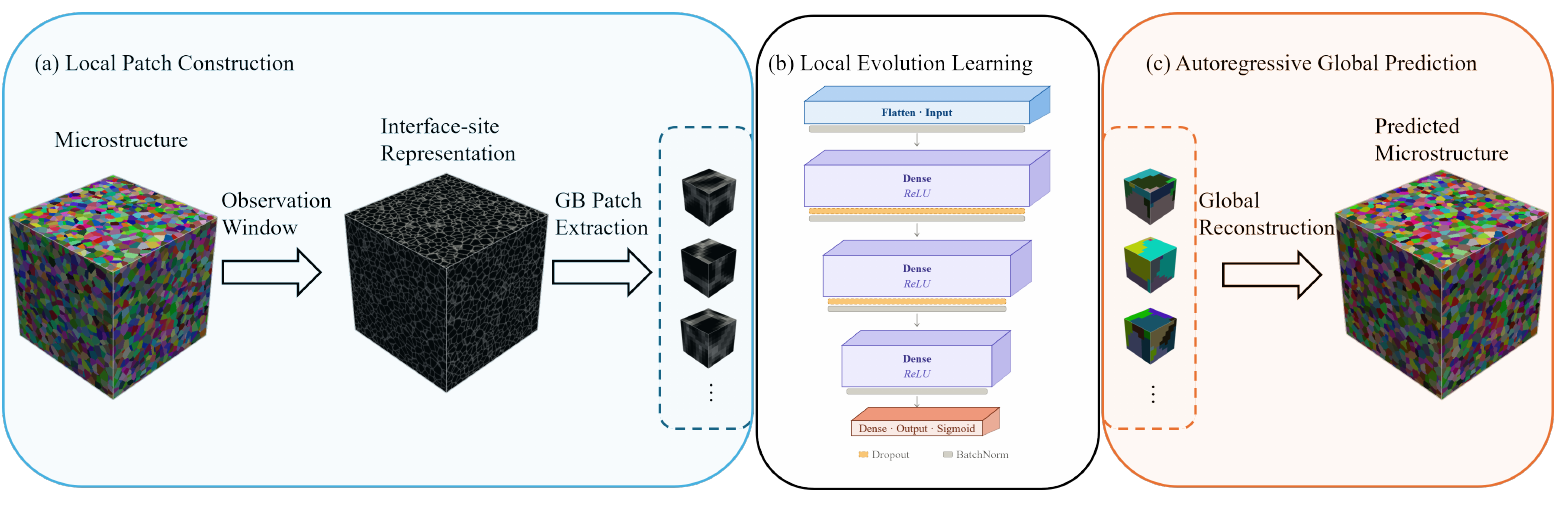
\includegraphics[alt={3D-PRIMME workflow from local grain-ID patches to autoregressive microstructure prediction},width=\textwidth]{figures/primme_workflow.png}
\caption{3D-PRIMME workflow: local patch construction from the grain-ID field, learning of local evolution scores, and autoregressive reconstruction of the global predicted microstructure. Adapted from Fig.~1 of the 3D-PRIMME manuscript.}
\label{fig:primme-workflow}
\end{figure}

Training and evaluation use three-dimensional MF data. The reported dataset contains 200 isotropic sequences and a corresponding set of inclination-dependent sequences. Each sequence starts from a different 512-grain Voronoi structure in a \(100^3\)-voxel volume and evolves for 100 simulation steps, while a training set uses only two consecutive states from one or more sequences. For the inclination-dependent data, the Gaussian sampling covariance is

\[
\boldsymbol{\Sigma}
=
\begin{pmatrix}
a & b & b\\
b & a & b\\
b & b & a
\end{pmatrix},
\qquad
a=25,\quad b=20,
\]

which biases the MF neighborhood along
\(\mathbf{u}_{111}=(1,1,1)/\sqrt{3}\). Between them, the isotropic and inclination-dependent datasets provide controlled teachers for testing whether the learned local operator recovers both scalar coarsening behavior and a prescribed directional response. No experimental microstructure is used in this completed study~\cite{tian2026threeDprimme}.

This covariance construction applies the neighborhood-design principle of Section~\ref{sec:neighborhood-physics} directly in three dimensions: the sampling distribution defines the directional response available to the surrogate. The completed studies do not contain a poor-versus-improved teacher ablation, but they do demonstrate the intended sequence from a diagnosed three-dimensional teacher to a learned anisotropic response.

\subsection{Completed performance}

\subsubsection{Local-context sensitivity and training variability.}

Window sensitivity tests show that all evaluated settings recover approximately linear coarsening, but the observation window affects the growth rate more strongly than the action window. The \(N_o=9\), \(N_a=9\) setting produces the smallest reported relative kinetic error, 2.85\%, and is used as the default. Ten replicate models trained on one two-state sequence show small spread in squared mean radius, average face count, topology-size relation, and voxel accuracy, although uncertainty grows with rollout time~\cite{tian2026threeDprimme}.

Two of the quantitative readouts can be written as

\begin{equation}
\begin{aligned}
\left\langle r(t)\right\rangle^2
&\approx
\left\langle r(0)\right\rangle^2+K_g t,\\
\operatorname{Acc}(t)
&=
\frac{1}{N}
\sum_{i=1}^{N}
\mathbf{1}\!\left[\hat{s}_i^{(t)}=s_i^{(t)}\right].
\end{aligned}
\label{eq:kinetics-accuracy}
\end{equation}

where the first relation is the parabolic coarsening diagnostic, \(K_g\) is the fitted growth-rate coefficient, and the second is voxel-wise agreement between predicted and reference grain labels. The coarsening relation is used as a kinetic diagnostic, not as a claim of universal continuous-time calibration.

\subsubsection{Spatial and temporal extrapolation.}

The distinction between training support and inference scale is central to 3D-PRIMME. The network is trained from local patches extracted from \(100^3\)-voxel volumes and requires only one transition between two consecutive states. During inference, the same fixed local operator is applied repeatedly and independently of the global domain dimensions. A model trained at \(100^3\) is applied without retraining to \(256^3\), \(512^3\), and \(1024^3\) domains containing approximately 8,600, 68,700, and 550,000 initial grains, respectively~\cite{tian2026threeDprimme}.

\begin{figure}[htbp]
\centering
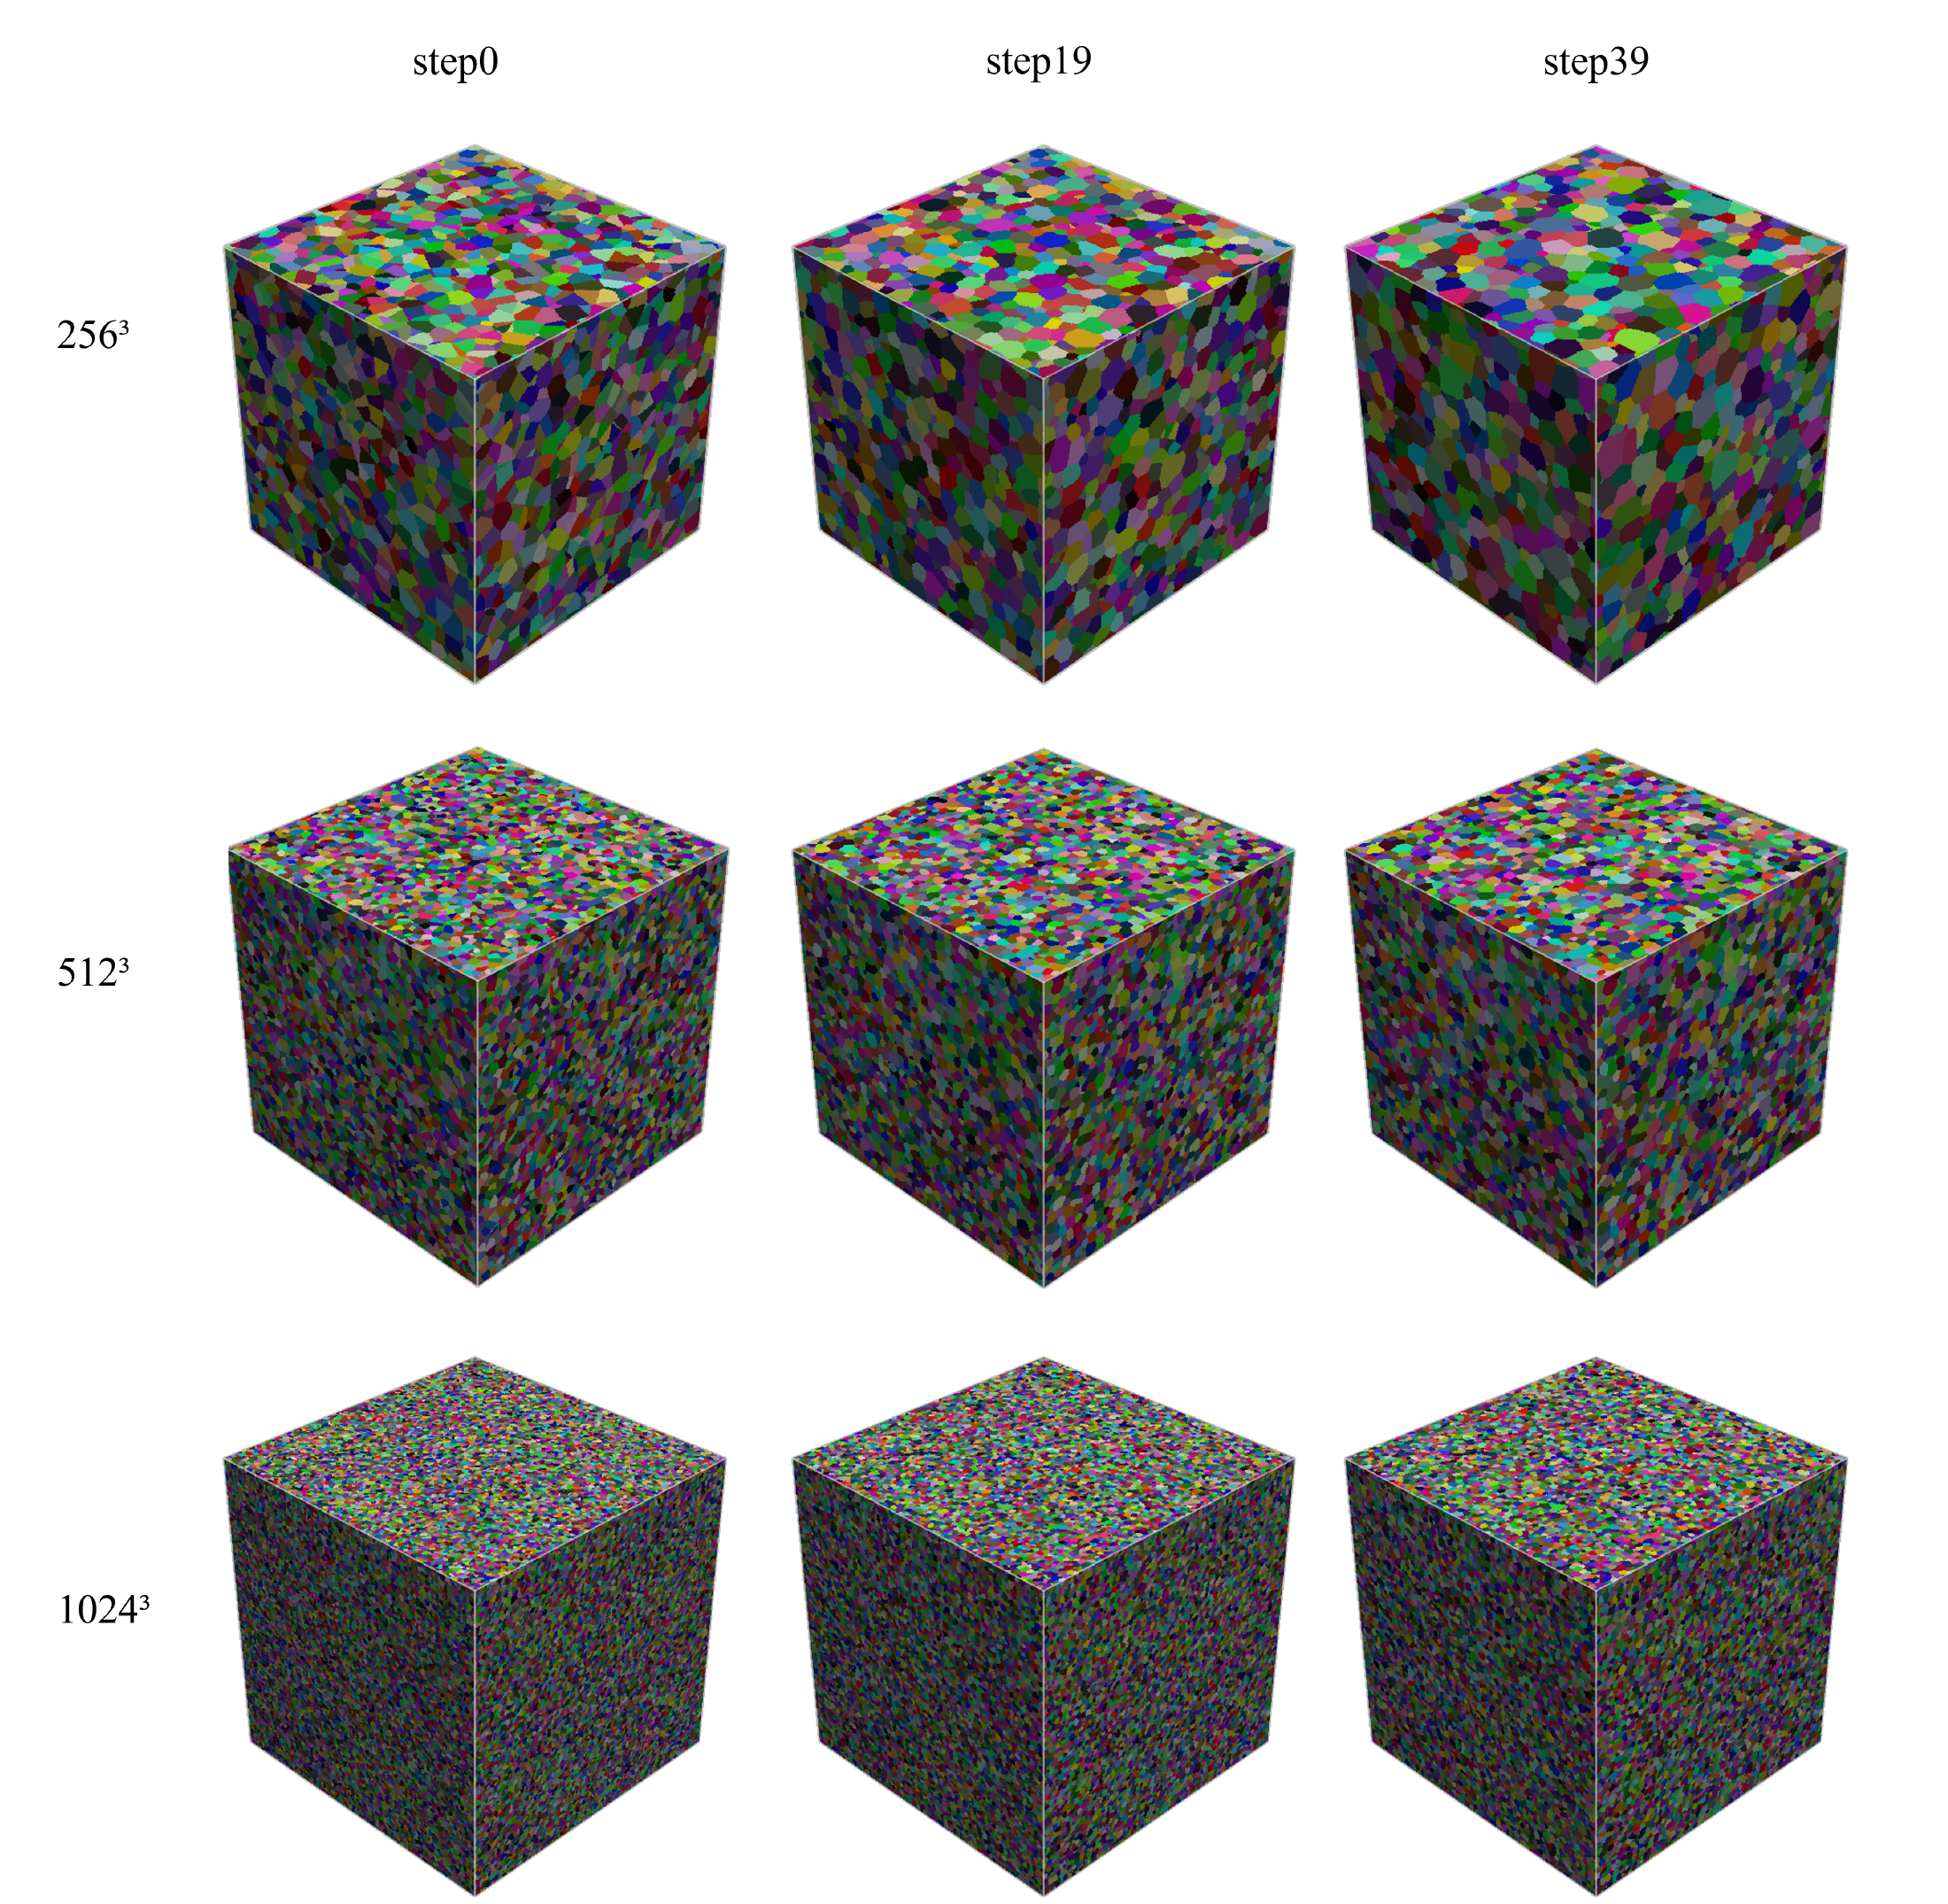
\includegraphics[alt={3D-PRIMME rollouts on 256 cubed, 512 cubed, and 1024 cubed voxel domains},width=0.96\textwidth]{figures/primme_spatial_extrapolation.png}
\caption{Visual evidence of spatial and temporal extrapolation by 3D-PRIMME. Representative \(256^3\), \(512^3\), and \(1024^3\) domains are shown at rollout steps 0, 19, and 39; the later states correspond approximately to one-half and one-quarter of the initial grain populations. The model was trained on \(100^3\) volumes and applied to all three larger domains without retraining. The cubes are displayed at a common visual size; row labels give the actual domain sizes. Adapted from Fig.~4 of the 3D-PRIMME manuscript.}
\label{fig:primme-extrapolation}
\end{figure}

The visual coarsening in Fig.~\ref{fig:primme-extrapolation} is accompanied by quantitative collapse across domain sizes. The tested scales exhibit closely overlapping squared-mean-radius trajectories, topological evolution, and normalized radius distributions at matched coarsening states. A \(1024^3\) rollout remains statistically stable for 100 steps, by which point 41,674 grains, or 7.6\% of the initial population, remain~\cite{tian2026threeDprimme}.

\begin{figure}[p]
\centering
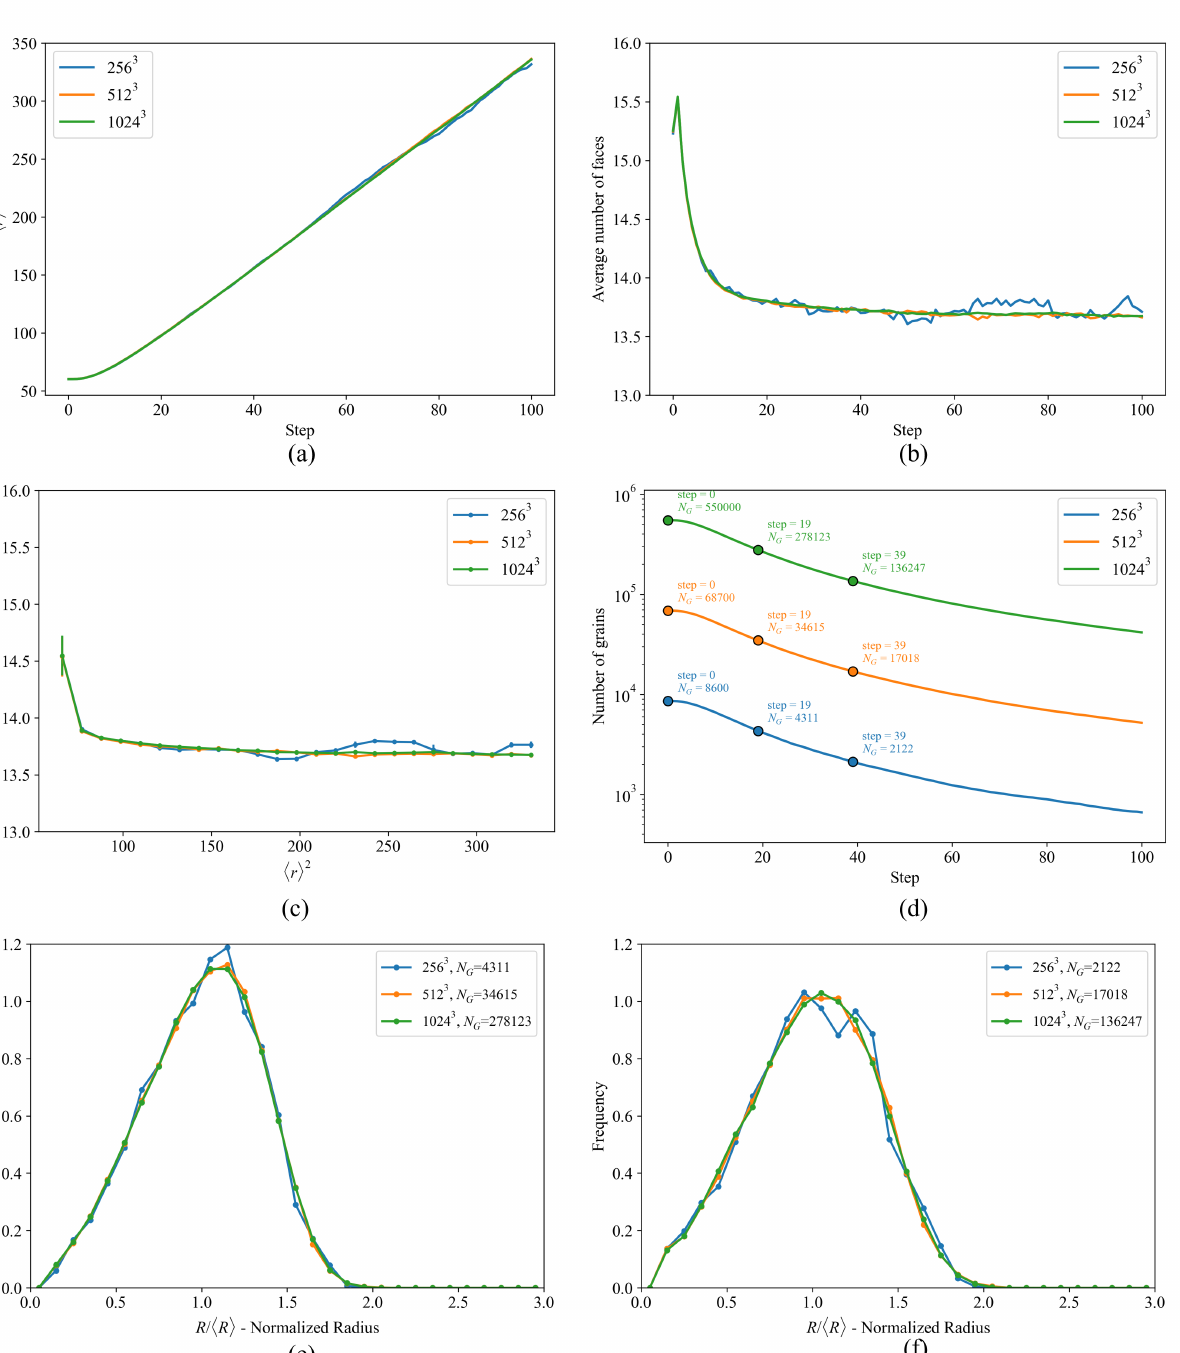
\includegraphics[
  alt={Kinetic, topological, grain-count, and grain-size statistics across three simulation domain sizes},
  width=\textwidth,
  height=0.80\textheight,
  keepaspectratio,
  trim=0 41 0 0,
  clip
]{figures/primme_spatial_scaling.png}
\par\vspace{-0.35\baselineskip}
\makebox[\textwidth][c]{%
  \makebox[0.49\textwidth][c]{\small (e)}%
  \makebox[0.49\textwidth][c]{\small (f)}%
}
\caption{Statistical consistency of 3D-PRIMME rollouts across \(256^3\), \(512^3\), and \(1024^3\) domains, including coarsening kinetics, topology, grain-count decay, and normalized grain-size distributions. Adapted from Fig.~5 of the 3D-PRIMME manuscript.}
\label{fig:primme-scaling}
\end{figure}

Together, Figs.~\ref{fig:primme-extrapolation} and~\ref{fig:primme-scaling} distinguish morphology from population-level fidelity: the first shows plausible three-dimensional evolution over increasing domain size, while the second shows that kinetic, topological, and distributional observables remain consistent. The demonstrated ``temporal extrapolation'' is autoregressive deployment beyond the two-state training interval within the MF setting; it is not a claim of calibrated physical-time prediction for an unseen material.

\subsubsection{Data efficiency under limited temporal supervision.}

Models trained on 1, 10, or 50 two-state sequences are evaluated against an independent set of ten MF simulations under a fixed number of optimizer updates. All three training-set sizes preserve approximately linear coarsening and similar face-count behavior. Ten sequences give the highest voxel accuracy and smallest replicate spread in that comparison, whereas the 50-sequence case coarsens more slowly and shows larger variability. The latter observation is treated as a training-design result, possibly reflecting redundancy, stochastic diversity, or insufficient optimization under the fixed update budget. It is not evidence that additional data are intrinsically harmful~\cite{tian2026threeDprimme}.

\subsubsection{Recovery of prescribed inclination dependence.}

The inclination-dependent test asks for more than recovery of scalar coarsening statistics. The anisotropic MF kernel produces an evolving directional signature, but boundary inclination is not supplied to 3D-PRIMME as an explicit input feature. Nevertheless, the initially near-circular distributions develop the expected elongated response, and the 3D-PRIMME curves remain close to the MF reference in the XY, XZ, and YZ projection planes through rollout step 50. This agreement indicates that the interface-site representation retains sufficient local geometry for the network to infer the teacher's direction-dependent update rule~\cite{tian2026threeDprimme}.

\begin{figure}[htbp]
\centering
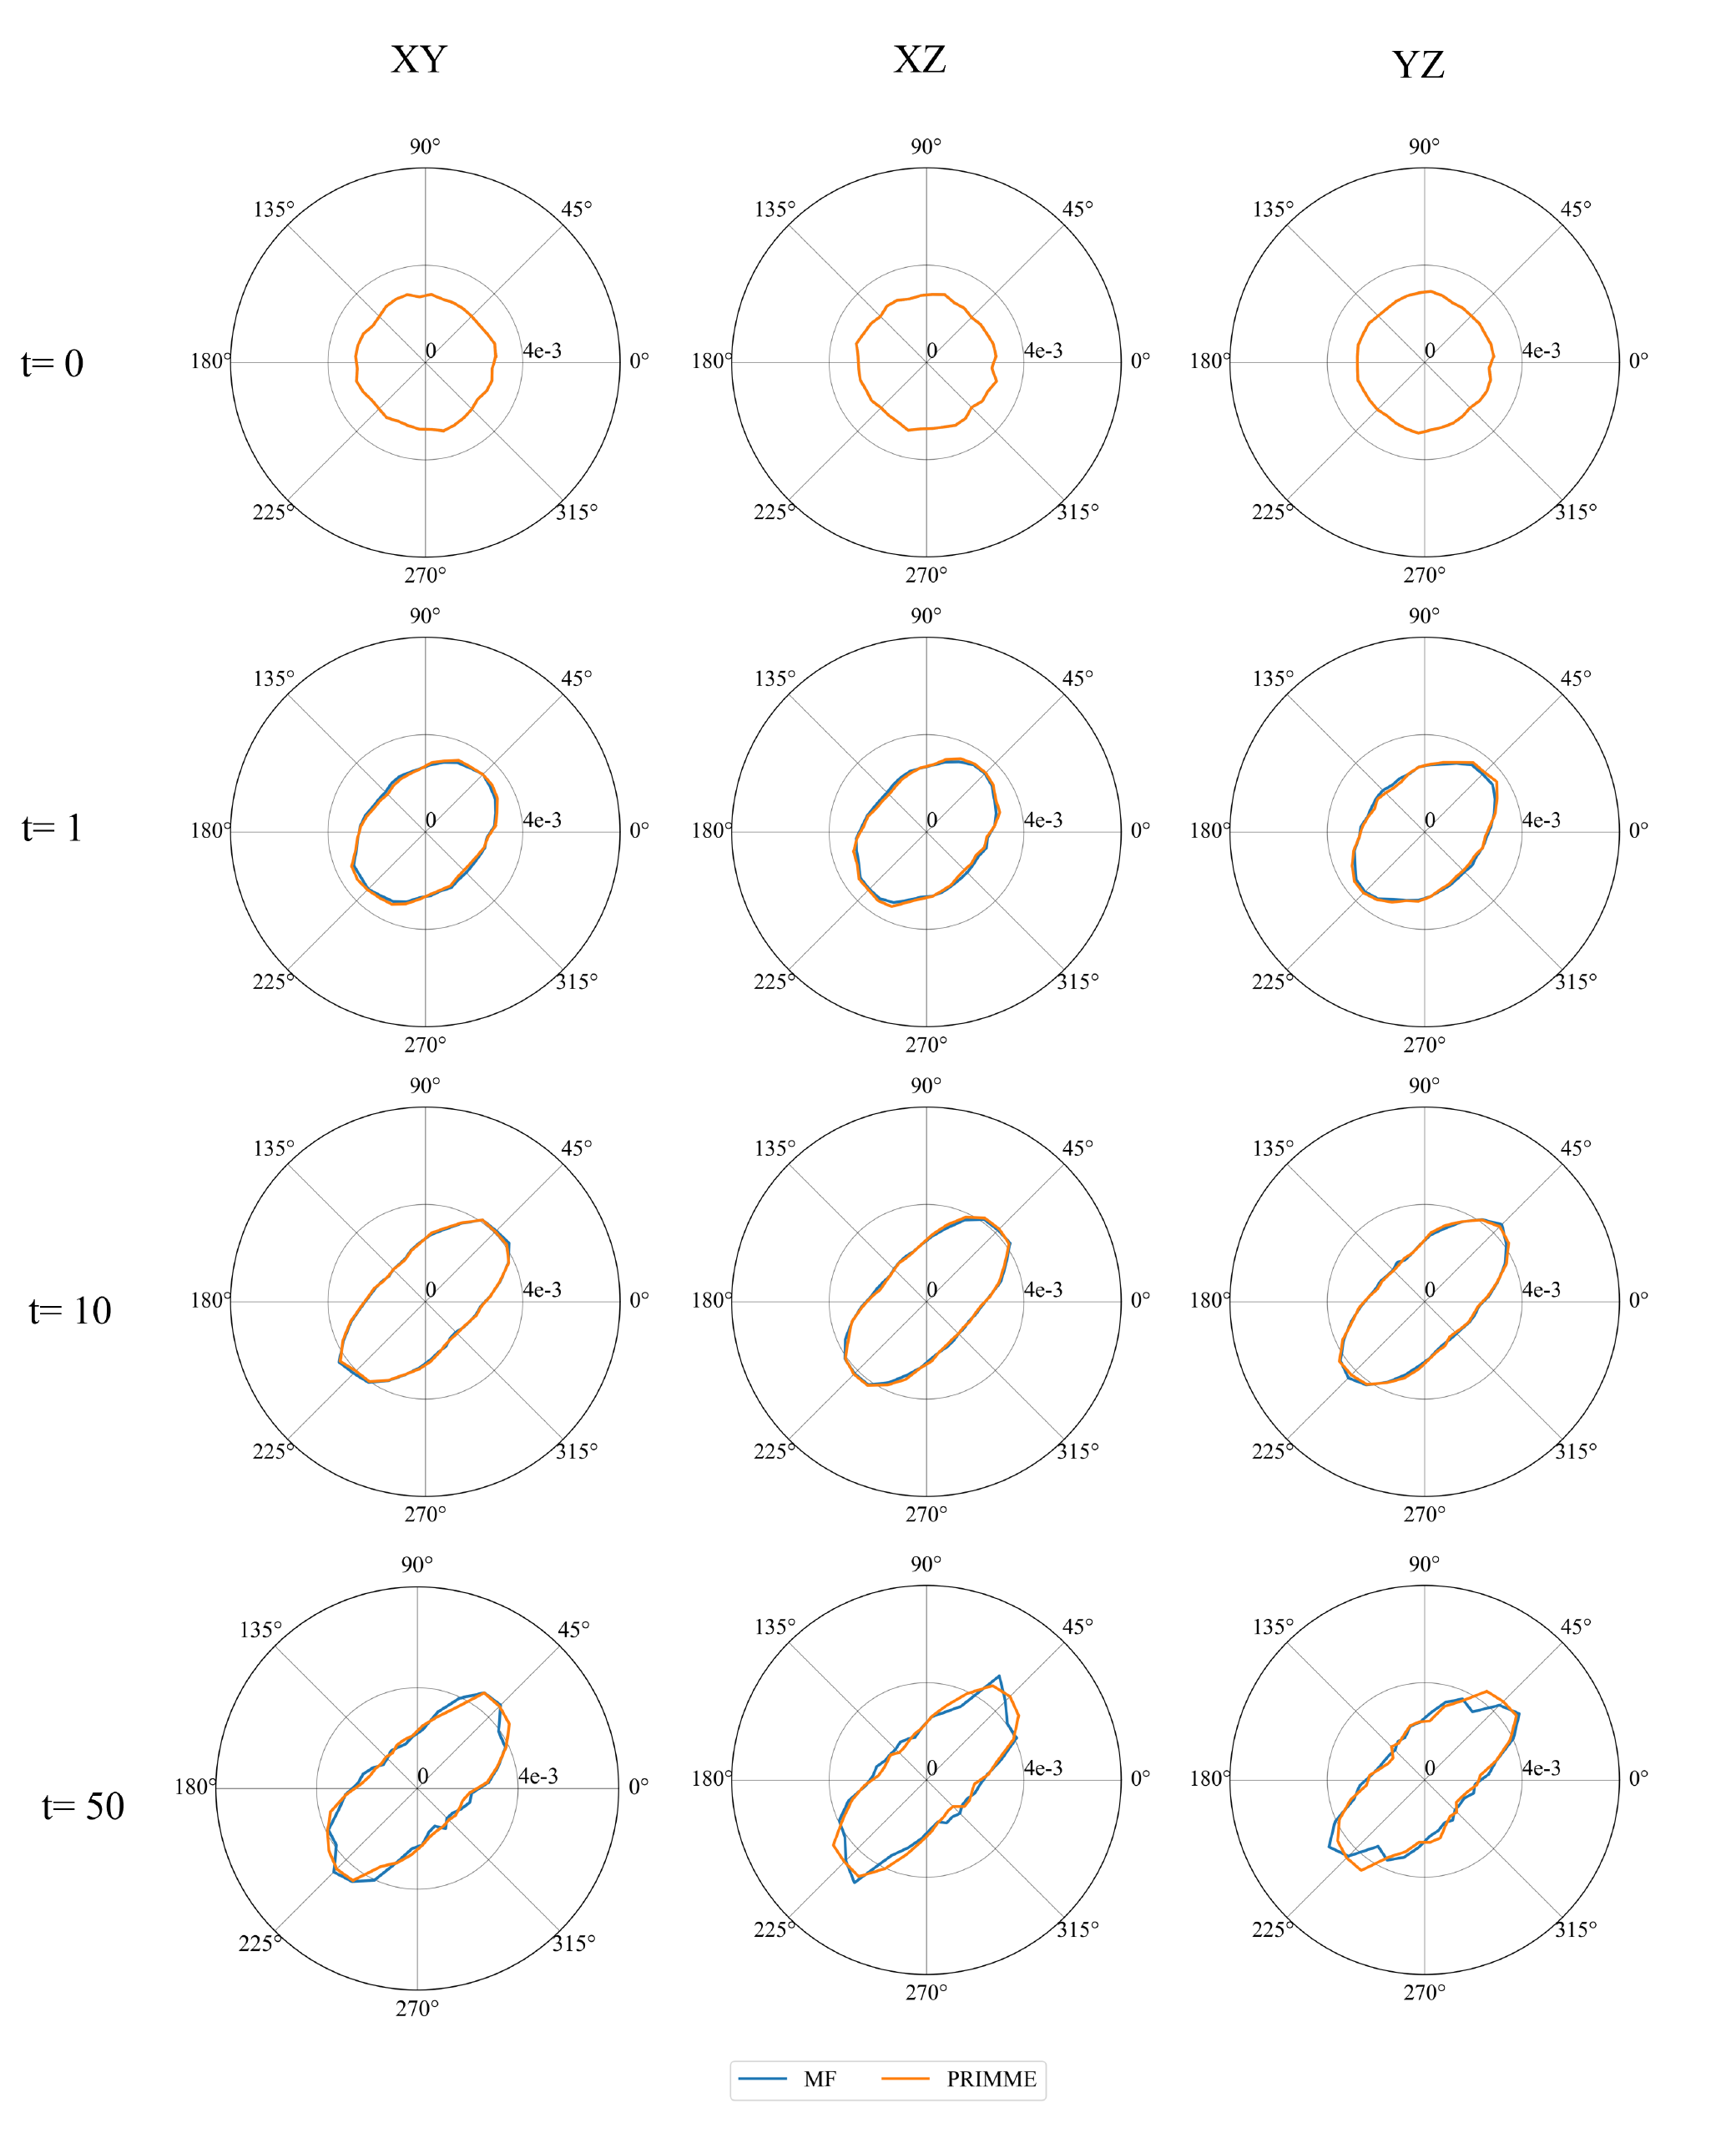
\includegraphics[alt={Reference and predicted inclination distributions in three projection planes over four rollout times},width=0.92\textwidth,height=0.78\textheight,keepaspectratio]{figures/primme_inclination_distributions.png}
\caption{Recovery of prescribed inclination dependence. MF reference distributions (blue) and 3D-PRIMME predictions (orange) are compared in the XY, XZ, and YZ projection planes at rollout steps 0, 1, 10, and 50. Agreement across the three projections shows that the model reproduces the directional response encoded by the anisotropic MF teacher even though inclination is not provided explicitly as an input. Adapted from Fig.~8 of the 3D-PRIMME manuscript.}
\label{fig:primme-inclination}
\end{figure}

\subsection{Scientific lesson and limitation}

The completed study demonstrates that a compact local representation contains sufficient information to reproduce major kinetic, topological, and inclination-dependent features of the MF teacher over spatial and temporal scales larger than those used for training. It also establishes that local context must be selected carefully: locality does not mean that an arbitrarily small or large neighborhood is equally informative.

The claim is nevertheless bounded by the supervision source. The model learns MF evolution, not universal grain-growth truth. Its geometry-only representation does not explicitly encode crystallographic misorientation, boundary energy, or mobility. Its successful recovery of anisotropy demonstrates learning of a prescribed simulation response, not discovery of an unknown experimental mechanism~\cite{tian2026threeDprimme}.

These limitations motivate the next stage. Once scalable local learning is technically feasible, the central question becomes whether the operator can be trained directly from measured evolution, where relevant behavior is not prescribed by a simulator.

\bigskip

\section{The reach and the ceiling of the completed foundations}

A simulation-trained surrogate is constrained twice: first by the simulator's representation of the material and then by the approximation error of the learned model. Improving agreement between 3D-PRIMME and MF reduces the second error but cannot remove the first. A high-fidelity surrogate of an idealized simulator remains an idealized model.

The completed studies make this distinction observable. The neighborhood work shows that local kernels can introduce, suppress, or prescribe inclination dependence. 3D-PRIMME then shows that a neural operator can recover the resulting simulated response. Together, they demonstrate both the strength and the ceiling of simulation supervision: controlled rules can be learned and scaled, but missing or incorrectly represented mechanisms cannot be recovered from labels that do not contain them.

Direct experimental learning matters because it tests whether measured evolution can supervise the same local architecture, not because it supplies additional patches. It changes the teacher from a prescribed stochastic model to measured microstructure evolution, and so removes the simulator from the label-generating path. This shift does \emph{not} by itself demonstrate that the experiment-trained operator has recovered material-specific physics absent from MF; establishing that difference would require a calibrated simulation--experiment comparison that is outside the core scope of this dissertation. Experimental labels also introduce uncertainty, incomplete observability, and acquisition artifacts. The next challenge is to determine whether those labels can support a reliable local operator without confusing measurement structure with physical evolution.

The completed simulation studies establish Levels 1--2 of Table~\ref{tab:evidence-ladder} relative to a controlled simulation teacher. They do not establish experimental Level 2 fidelity or Levels 3--5. The experimental work and proposed aims retain this same hierarchy: each stronger claim is conditional on the evidence required at the preceding level.


\chapter{Experimental Foundation and Remaining Research Gap}

The current five-state laboratory-DCT volume is the only experimental dataset assumed available for core dissertation completion. A second specimen, additional thermal history, or additional time state is not required by the proposed plan and is not presently used to support a generalization claim. Data ownership, the practical availability of additional measurements, and permission to release curated derivatives remain to be confirmed.

\section{Challenges of learning from sparse 4D experiments}

\subsection{Structured label uncertainty}

Experimental grain-ID maps are not automatically valid training pairs. Rigid translation and rotation produce apparent boundary displacement. Residual non-rigid distortion can create a spatially varying update field. Surface recession changes the common material volume. Grain identities can be lost or incorrectly linked between scans. Small grains may fall below detection thresholds, and segmentation churn can create or remove apparent grains. If these effects are passed directly to an autoregressive model, the network can learn them as spurious dynamics~\cite{tian2026experiment}.

Label-preserving preprocessing is part of the scientific method here. Continuous interpolation is inappropriate for categorical grain identities because it produces values that do not correspond to grains. Registration must move whole labels, preserve identity, and expose residual uncertainty instead of hiding it through smoothing.

Unlike independent label noise, these effects can produce a spatially organized apparent update rule that is repeatedly amplified during autoregressive rollout. Direction-sensitive registration residuals and rollout drift are therefore as important as aggregate fit metrics.

\begin{figure}[htbp]
\centering
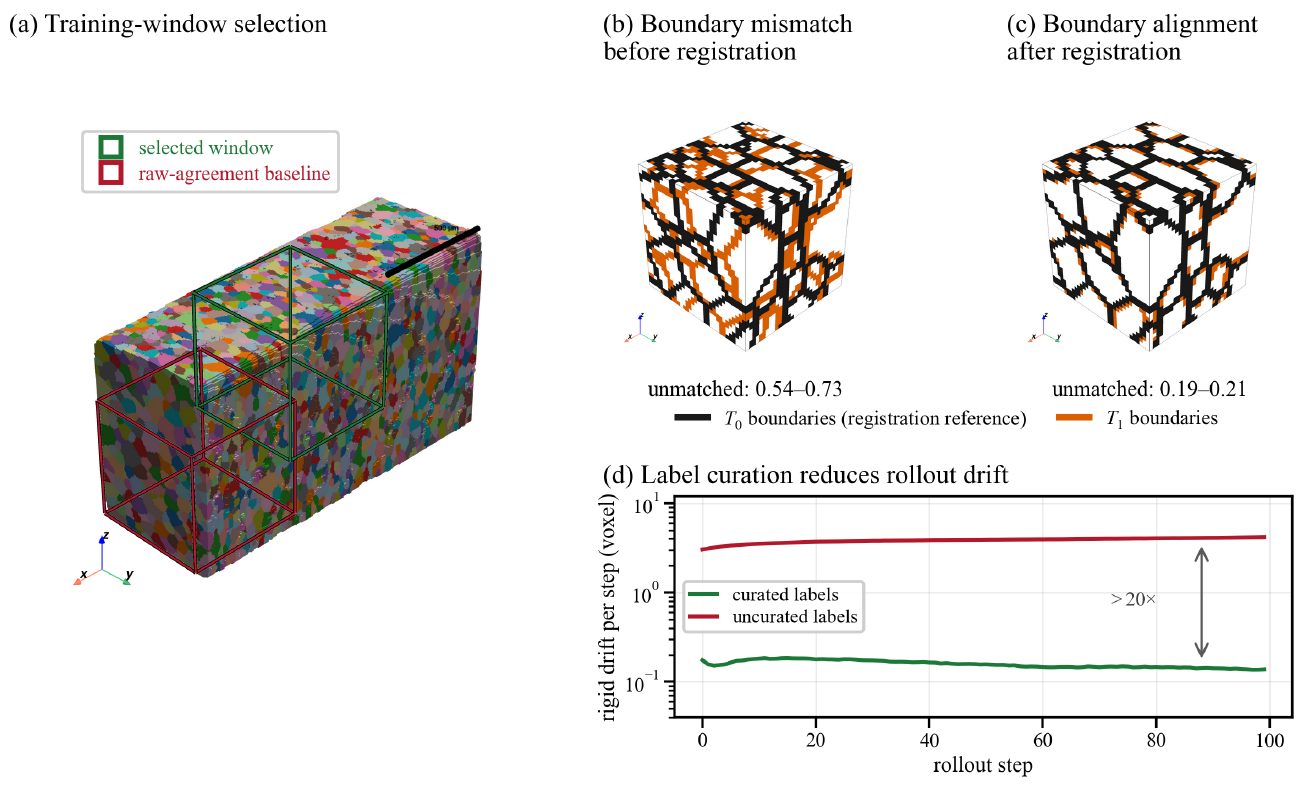
\includegraphics[alt={Experimental window selection, boundary registration, and reduction of rollout drift after label curation},width=0.95\textwidth]{figures/experiment_curation.png}
\caption{Experimental-label curation and its diagnostics: residual-driven training-window selection, boundary mismatch before and after integer registration, and the reduction in learned rollout drift after curation. Adapted from Fig.~1 of the Experimental surrogate manuscript.}
\label{fig:experimental-curation}
\end{figure}

\subsection{Spatial abundance and temporal scarcity}

Non-destructive X-ray grain mapping has progressed from synchrotron structural microscopy and direct observations of bulk-grain evolution to synchrotron and laboratory diffraction-contrast tomography~\cite{larson2002xray,schmidt2004watching,ludwig2008dct,king2013labdct,mcdonald2015labdct}. These methods now supply voxelized three-dimensional grain maps at successive states and have enabled time-resolved studies of grain growth and related microstructural evolution~\cite{mckenna2014fourD,mcdonald2017sintering,zhang2018grain,wang2025abnormal}. The present dataset is spatially rich but temporally sparse: one pair of volumes contains hundreds of thousands of local boundary-centered patches, but the dataset contains only five independent time states. This asymmetry makes local learning feasible while limiting claims of generalization. Overlapping patches from one transition increase the optimization sample count, but they do not replace independent experimental windows or time intervals. Random voxel-level train/validation splits test whether the architecture fits the selected pair; they do not demonstrate cross-window or cross-material transfer, consistent with the known optimism of random validation when samples retain spatial or temporal dependence~\cite{roberts2017crossvalidation,tian2026experiment}.

The correct unit of future validation is the experimental partition: a window, a time pair, a spatial block, or a linked grain, and not an individual overlapping voxel. Aim 1 is designed around this principle.

\subsection{Multilevel validation}

Experimental reliability cannot be decided with one scalar score. The current study shows why. Grain-size distributions can agree while topology remains biased; an apparently stable rollout can miss late experimental slowdown; aggregate coarsening can be plausible while individual-grain magnitude is underpredicted. Most directly, a model trained on the same experimental window without label curation retained plausible population-level statistics while its recursive rollout developed a coherent rigid translation of approximately \(3.5\) voxels per step (Fig.~\ref{fig:experimental-curation}). Directional drift reveals a learned registration artifact that aggregate statistics miss. The proposed work will preserve a multilevel evaluation matrix instead of collapsing all outcomes into a single accuracy number~\cite{tian2026experiment}.

This multilevel strategy is consistent with the distinction between aleatoric and epistemic uncertainty in machine learning, practical ensemble-based uncertainty estimation, and evidence that both dataset shift and autoregressive rollout require assessment beyond one-step fit~\cite{hullermeier2021uncertainty,lakshminarayanan2017ensembles,ovadia2019shift,mccabe2023stability}. It also reflects simulation--experiment comparisons and experimental grain-growth studies showing that size statistics, topology, curvature, boundary character, and measured grain-volume change need not reduce to one scalar relation~\cite{mckenna2014fourD,rowenhorst2010topology,martine2019metrics,bhattacharya2021curvature,peng2022comparison,rohrer2011anisotropy,han2018kinetics}.

\bigskip

\section{Experimental data curation and direct training}

\textbf{Research status: ONGOING WORK WITH STABLE PRELIMINARY RESULTS}

\subsection{Experimental data and curation}

The ongoing study uses a five-state laboratory DCT grain-growth dataset. The full reconstruction contains \(549\times149\times211\) voxels. A candidate \(100^3\) analysis window is selected through a residual-driven search and then trimmed in place to \(100\times95\times84\) voxels so that all registered states remain inside the material. The window contains 1,757 grains initially and 1,345 grains after four intervals, while the reported mean radius increases by approximately 10\%~\cite{tian2026experiment}.

Window selection is based on post-registration residual and displacement-gradient amplitude, not on raw inter-frame agreement. The selected window ranks 15th among 831 candidates under that objective, whereas the raw-agreement baseline ranks last. Registration uses a rounded affine displacement field so that whole categorical grain labels are copied without interpolation. This reduces unmatched boundary fractions on three visible faces from 0.54-0.73 to 0.19-0.21 and leaves residual displacement no larger than 0.05 voxel per axis. The curation removes 87\% of the dominant rotation-induced displacement ramp and trims the analysis volume to remain interior as the surface recedes~\cite{tian2026experiment}.

The integer displacement applied at voxel position \(\mathbf{x}\) is

\begin{equation}
\boldsymbol{\delta}(\mathbf{x})
=
\operatorname{round}
\left[
\boldsymbol{\phi}
+\mathbf{G}\left(\mathbf{x}-\mathbf{c}\right)
\right],
\label{eq:integer-registration}
\end{equation}

where \(\boldsymbol{\phi}\) is the remeasured fractional offset, \(\mathbf{G}\) is the fitted displacement-gradient tensor, and \(\mathbf{c}\) is the window center. Componentwise rounding ensures that registration copies existing categorical labels instead of synthesizing interpolated grain identities.

Grain identities are linked between full-volume frames before registration using greedy one-to-one maximum-overlap matching. For the training pair, 90.4\% of T1 grains and 97.4\% of T1 voxels inherit T0 identities. The remaining 2.6\% of T1 voxels generate all-zero target maps instead of fabricated identity assignments~\cite{tian2026experiment}.

\subsection{Direct experimental training}

The unmodified 3D-PRIMME architecture is trained on the T0-to-T1 transition. A \(9^3\) observation and \(9^3\) action neighborhood yield 729 input/output features per boundary-centered sample. The training pair supplies 797,712 local samples, split randomly 80/20 for optimization monitoring, and three independent models are trained from different initializations. T2-T4 are held out from fitting, although all five frames are used to define the common interior field of view~\cite{tian2026experiment}.

The experiment-trained model uses the same interface representation, candidate-update target, and squared-error loss defined in Equations~\eqref{eq:primme-representation}--\eqref{eq:primme-loss}; for this training pair, \(t=0\) and \(t+1=1\) correspond to T0 and T1. The mathematical operator is unchanged, while the grain-ID fields supplying \(S_i^{(t)}\) and \(y_{ij}^{(t)}\) now come from curated measurements instead of MF simulation.

This design establishes direct-training feasibility. It does not yet establish spatial reproducibility beyond the selected window because all fitting samples come from one field of view, nor complete temporal independence because later frames contribute to the common-volume definition.

The uncurated direct-training control provides a particularly important negative result. Despite apparently consistent population-level statistics, recursively applying the learned operator produces a coherent rigid drift of \(3.0\)--\(4.2\) voxels per step, with a mean near \(3.5\) voxels per step (Fig.~\ref{fig:experimental-curation}). The model can pass selected statistical checks while learning scan displacement as if it were grain-growth dynamics. After label curation, the mean per-step drift across the three models is approximately \((-0.02,+0.13,-0.09)\) voxels along \((x,y,z)\); for the representative rollout, the drift magnitude remains bounded at approximately \(0.14\)--\(0.18\) voxel per step, more than twenty times below the uncurated control. The residual direction is consistent with the known rotational shear. Statistical agreement alone is not enough: directional, field-level rollout diagnostics must accompany aggregate accuracy~\cite{tian2026experiment}.

\section{Stable preliminary results}

The learned rollouts remain visually coherent over the experimental window. Large grains grow, small grains disappear, boundaries flatten, and only a short-lived single-voxel speckle artifact is reported. Early aggregate coarsening is also reproduced: after one rollout step, the representative prediction retains 1,624 grains compared with 1,609 in experiment. This one-step comparison has not yet been benchmarked against a no-change or persistence predictor and remains preliminary. The prediction then diverges as the experiment slows between T3 and T4 while the fixed two-hour learned operator maintains a steadier rate. The manuscript does not establish a continuous-time calibration~\cite{tian2026experiment}.

\begin{figure}[htbp]
\centering
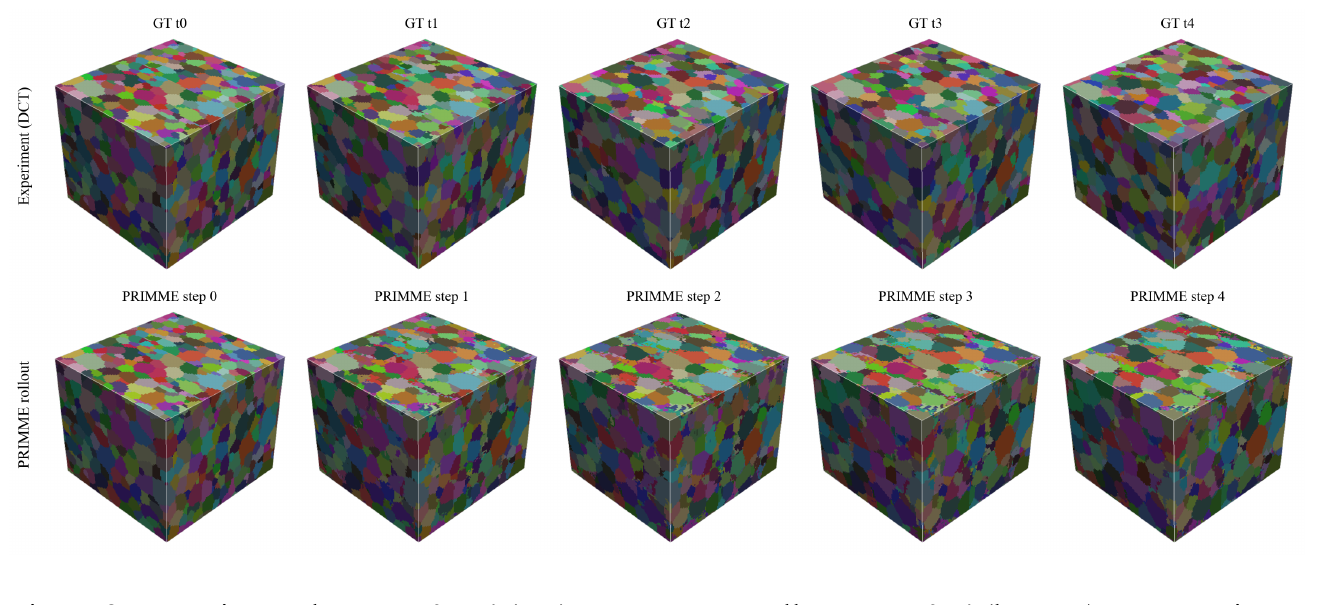
\includegraphics[alt={Experimental grain maps T0 through T4 above corresponding experiment-trained rollout states},width=0.98\textwidth]{figures/experiment_rollout.png}
\caption{Experimental states T0--T4 (top) and the corresponding experiment-trained PRIMME rollout steps 0--4 (bottom), shown with a shared grain-ID color map for one representative replicate. Adapted from Fig.~2 of the Experimental surrogate manuscript.}
\label{fig:experimental-rollout}
\end{figure}

\begin{figure}[htbp]
\centering
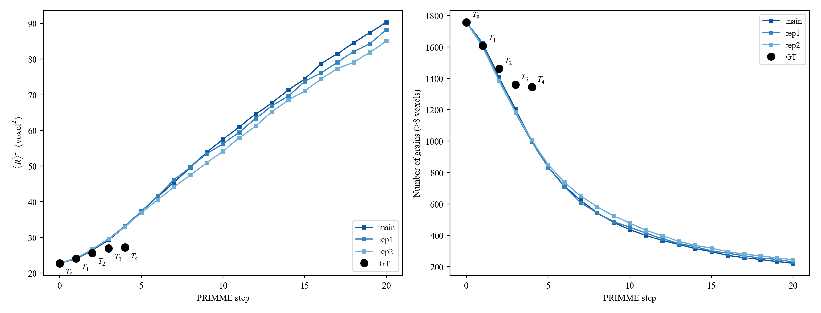
\includegraphics[alt={Mean squared grain radius and grain-count trajectories for experiment and three model replicates},width=0.98\textwidth]{figures/experiment_metric_coarsening.pdf}
\caption{Experimental and experiment-trained coarsening trajectories. Left: mean squared grain radius. Right: number of grains larger than eight voxels. Three independently trained replicates are compared with experimental states T0--T4. Extracted as vector artwork from Fig.~3 of the Experimental surrogate manuscript.}
\label{fig:experimental-coarsening}
\end{figure}

Normalized grain-size distributions show encouraging held-out agreement. For normalized radius \(z=R/\langle R\rangle\), the reported two-sample Kolmogorov-Smirnov statistic is

\begin{equation}
D_{\mathrm{KS}}
=
\sup_z
\left|
\widehat{F}_{E}(z)
-\widehat{F}_{\widehat{E}}(z)
\right|,
\label{eq:ks}
\end{equation}

where \(\widehat{F}_{E}\) and \(\widehat{F}_{\widehat{E}}\) are the empirical cumulative distributions for the experimental reference and the experiment-trained rollout at matched grain count. Across three later states and three model replicates, reported \(D_{\mathrm{KS}}\) values range from 0.071 to 0.095. When analysis is restricted to grains larger than the approximately \(20\,\mu\text{m}\) experimental confidence limit, the values decrease to 0.025-0.059. Because the experiment slows, all later frames are paired with rollout step 2 under the matched-grain-count analysis. The resulting nine distances do not represent nine independent rollout states. In addition, a persistence or other prespecified null distribution has not yet been reported. These comparisons support preliminary distribution-shape consistency, but their incremental value over a self-similar or unchanged-distribution baseline remains to be quantified~\cite{tian2026experiment}.

\begin{figure}[htbp]
\centering
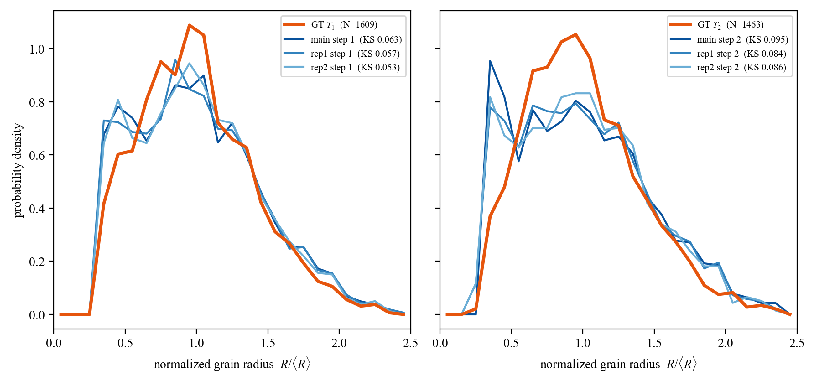
\includegraphics[alt={Normalized grain-size distributions for a trained state and a held-out experimental state},width=0.98\textwidth]{figures/experiment_metric_size_distribution.pdf}
\caption{Normalized grain-size distributions at matched grain count. Left: the trained state T1. Right: the T2 held-out state with the largest reported Kolmogorov--Smirnov distance. The experimental distribution is compared with three independent model replicates. Extracted as vector artwork from Fig.~4 of the Experimental surrogate manuscript.}
\label{fig:experimental-size-distribution}
\end{figure}

Topology reveals a clear current limitation. At rollout steps paired with the held-out states, predicted face counts remain above the experimental band. Transient arg-max speckle and sensitivity to small grains are candidate explanations, not established causes; Aim 1 will test them through readout and speckle-sensitivity analyses. Individual-grain analysis is feasible only where identity linkage remains sufficiently reliable: growth/shrinkage sign accuracy is 72-73\% on the training interval and 62-63\% on the usable T2-to-T3 held-out interval, with regression slopes of 0.78 and 0.57, respectively. The majority-class growth/shrinkage baseline has not yet been reported, so the incremental information in sign accuracy remains to be established. The fitted slopes nevertheless show that the current model underpredicts the magnitude of grain-volume change~\cite{tian2026experiment}.

\begin{figure}[htbp]
\centering
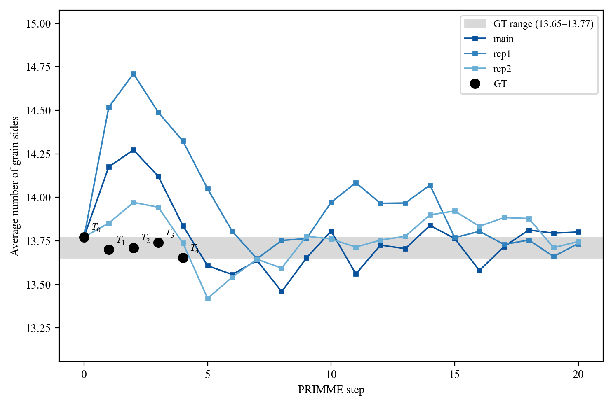
\includegraphics[alt={Mean faces per grain for three model rollouts relative to the experimental range},width=0.98\textwidth]{figures/experiment_metric_topology.pdf}
\caption{Mean faces per grain during the experiment-trained rollout. The gray band gives the range across the five experimental states; all three predicted trajectories remain above this range at the steps paired with held-out measurements. Extracted as vector artwork from Fig.~5 of the Experimental surrogate manuscript.}
\label{fig:experimental-topology}
\end{figure}

\begin{figure}[htbp]
\centering
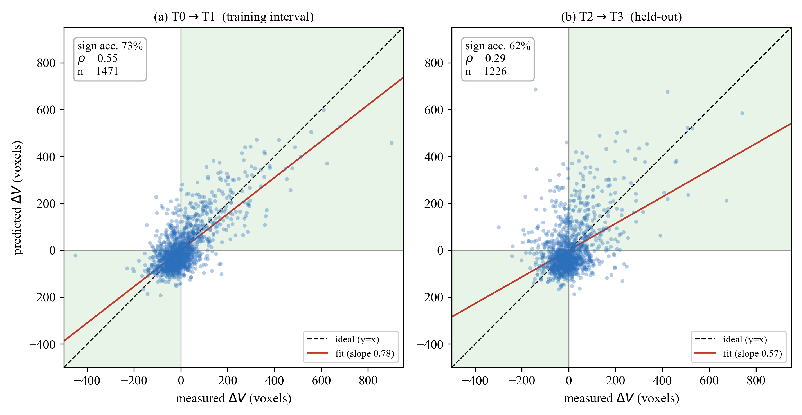
\includegraphics[alt={Predicted versus measured grain-volume changes for training and held-out intervals},width=0.98\textwidth]{figures/experiment_metric_grain_response.pdf}
\caption{Linked grain-by-grain volume change for the T0-to-T1 training interval (left) and the usable T2-to-T3 held-out interval (right). Shaded quadrants indicate correct growth/shrinkage sign; dashed lines show ideal agreement and red lines show least-squares fits. Extracted as vector artwork from Fig.~6 of the Experimental surrogate manuscript.}
\label{fig:experimental-grain-response}
\end{figure}

A 100-step extrapolation remains numerically stable and decreases monotonically to 38 grains, but this long rollout has no experimental reference and is not treated as physical validation~\cite{tian2026experiment}.

\section{Remaining gap motivating the proposed aims}

The stable results establish direct-training feasibility and Level 1 evidence in the selected field of view. The remaining limitations fall into two groups.

\subsection*{Gaps addressed by this proposal}
\begin{itemize}

\item \textbf{Reliability across experimental partitions (Aim 1):} determine whether curation quality and model behavior reproduce across prespecified windows and spatial/temporal blocks within the available volume.

\item \textbf{Meaningful experimental baselines and topology diagnostics (Aim 1):} compare model performance with persistence and majority-class nulls and test whether readout, speckle, and small-grain sensitivity account for the observed topology bias.

\item \textbf{Training-blind system validation (Aim 2):} apply the definitions and null baselines frozen in Aim 1, without modification, to an experimental partition that contributed to neither training nor model selection, and adjudicate each metric family once.

\item \textbf{Interpretability and physics learning (Aim 3):} determine which spatial information a validated experiment-trained model uses and how that information is converted into local evolution decisions; symmetry-audited scale and Jacobian analyses are the probes currently developed.

\end{itemize}

\subsection*{Limitations not resolved or not guaranteed by this proposal}
\begin{itemize}

\item cross-specimen, cross-processing-condition, or cross-material generalization;

\item a continuously calibrated physical-time evolution law or guaranteed correction of late-time kinetics;

\item formal probabilistic uncertainty calibration if the number of sufficiently independent windows is inadequate;

\item proof that experimental supervision contains specific material physics absent from MF, which would require a separately calibrated simulation--experiment comparison;

\item unique physical-mechanism discovery; Aim 3 may instead establish stable model interpretation or bounded physical attribution.

\end{itemize}


\chapter{Proposed Research: Specific Aims}

The remaining research is organized by scientific dependency, not by manuscript. Aim 1 establishes when experimental learning is trustworthy within the available volume. Aim 2 converts those frozen definitions into a single confirmatory test on an experimental partition that was never used for training or model selection. Aim 3 will interpret only relationships that survive the applicable evidence gates.

\begin{figure}[htbp]
\centering
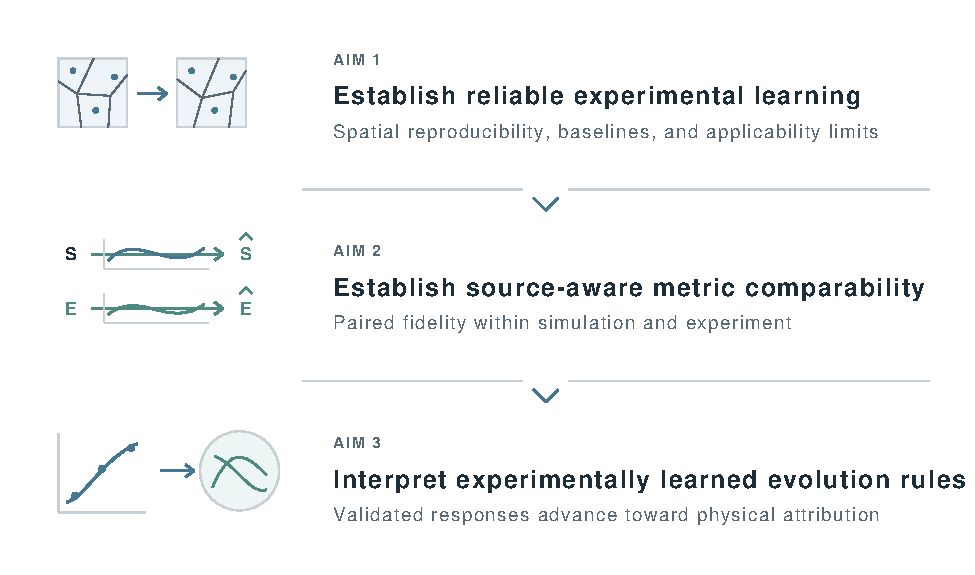
\includegraphics[alt={Dependency ladder in which Aim 1 enables Aim 2 and Aim 2 enables Aim 3},width=0.94\textwidth]{figures/specific_aims_overview.pdf}
\caption{Specific Aims and their scientific dependency. Reliability established in Aim 1 enables training-blind system validation in Aim 2; only validated relationships advance to interpretability and physics learning in Aim 3.}
\label{fig:specific-aims-overview}
\end{figure}

\section{Aim 1: Establish reliable learning across sparse 4D experimental windows}

\textbf{Status:} Single-window results are stable preliminary evidence; multi-window analysis is ongoing; core reliability and empirical uncertainty analysis are proposed.

\subsection{Scientific question}

Under what curation, registration, linkage, training, and validation conditions can an experiment-trained local surrogate be trusted across prespecified partitions of the available experimental volume?

\subsection{Hypothesis}

If voxel-level labels are curated with direction-sensitive registration checks and evaluated across grouped experimental windows and temporal partitions, then experiment-trained local operators will exhibit measurable spatial reproducibility at field, population, topology, and individual-grain levels within a definable domain of applicability. Empirical variability arising from window selection, model initialization, and key curation choices should increase under less-supported conditions and identify cases in which prediction must be qualified or withheld.

\subsection{Rationale}

The current experimental manuscript establishes direct-training feasibility but not spatial reproducibility beyond one selected window. All training data originate from one field of view and one two-hour transition. Three initialization replicates characterize optimization variability, while threshold, padding, drift, and readout analyses reveal several single-window sensitivities. Adding further diagnostics to that window would not settle the question. What is needed is a test of whether the learned operator and its conclusions reproduce across experimentally meaningful partitions of the available volume, without presenting same-specimen windows as cross-material generalization.

\subsection{Completed preliminary evidence}

Stable preliminary evidence includes residual-driven window selection, whole-label integer registration, interior-volume trimming, grain linkage, direct T0-to-T1 training, three model replicates, held-out T2-T4 evaluation, grain-size and topology comparisons, individual-grain tests where linkage permits, and directional rollout-drift analysis. These results establish feasibility and provide the baseline metrics for the proposed multi-window work~\cite{tian2026experiment}. Table~\ref{tab:aim1-preliminary-proposed} separates what they already show from what Aim 1 adds.

\begin{table}[htbp]
\centering
\caption{Boundary between stable preliminary results and proposed Aim 1 extensions.}
\label{tab:aim1-preliminary-proposed}
\small

\begin{tabularx}{\textwidth}{@{}*{3}{>{\raggedright\arraybackslash}X}@{}}

\toprule

\textbf{Dimension} & \textbf{Stable preliminary work} & \textbf{Aim 1 extension} \\

\midrule

Spatial coverage & One curated experimental window & Multiple prespecified windows from the current volume \\

Replication & Three model initializations & Variability across windows, models, and key curation choices \\

Validation & Later states in the same field of view & Grouped spatial and temporal validation \\

Sensitivity & Detection threshold, padding, drift, and readout within one window & Cross-window robustness and domain of applicability \\

Scientific claim & Feasibility of direct experimental training & Spatial reproducibility and domain of applicability within the available volume \\

\bottomrule
\end{tabularx}
\end{table}

\subsection{Proposed methodology}

\textbf{1. Quantify window feasibility before model comparison.} The full reconstruction is \(549\times149\times211\) voxels and candidate windows are selected at \(100^3\) voxels before trimming. Table~\ref{tab:window-geometry} gives the geometric support available for window placement. Because the \(y\) extent is only 149 voxels, any two \(100\)-voxel candidate windows must overlap by at least 51 voxels in \(y\). The absolute packing bound is ten mutually non-overlapping \(100^3\) windows, and no partition can be described as independent merely because it contains a different window origin. The actual candidate stride, overlap graph, quality distribution, and admissible-window count will be recorded before the partition design is frozen.

\begin{table}[htbp]
\centering
\caption{Geometric constraints on placing \(100^3\) candidate windows in the available DCT volume. The start-position range is inclusive.}
\label{tab:window-geometry}
\small
\begin{tabularx}{\textwidth}{@{}*{5}{>{\raggedright\arraybackslash}X}@{}}
\toprule
\textbf{Axis} & \textbf{Volume extent} & \textbf{Window extent} & \textbf{Start-position range} & \textbf{Maximum non-overlapping count} \\
\midrule
\(x\) & 549 & 100 & 0--449 & 5 \\
\(y\) & 149 & 100 & 0--49 & 1 \\
\(z\) & 211 & 100 & 0--111 & 2 \\
\bottomrule
\end{tabularx}
\end{table}

\textbf{2. Define a minimum multi-window dataset.} Additional candidate windows will be selected from the current DCT volume using the same residual-driven philosophy as the preliminary study. Selection criteria will be fixed before model comparison and will include interior-volume support, post-registration residual, displacement-gradient amplitude, boundary content, and linkage feasibility. The final number and placement of windows will depend on their measured quality.

\textbf{3. Apply a consistent label-preserving curation pipeline.} Each selected window will undergo whole-label integer registration, in-place trimming to a common interior volume, and full-volume grain linkage. Registration residuals, unmatched boundary fractions, linkage yield, and retained volume will be recorded, not buried as preprocessing detail.

\textbf{4. Define grouped training and validation partitions.} Windows connected by spatial overlap will remain in the same block so that overlapping voxels do not create an artificial impression of independence. The effective sample size will be reported at the window or non-overlapping block level rather than as the number of candidate origins or voxel patches. Because independent blocking in \(y\) is geometrically impossible at the candidate-window scale, primary spatial holdouts will be defined along supported \(x\) and \(z\) separations, with overlapping-window analyses labeled as sensitivity or reproducibility tests, not as independent validation. Temporal holdout will be retained where common-volume and linkage definitions permit it.

\textbf{5. Train replicate local operators under fixed definitions.} The core architecture, observation/action windows, optimizer settings, readout, and replicate policy will be held fixed for the primary comparison. Broad architecture or hyperparameter sweeps are optional and will not displace the multi-window analysis.

\textbf{6. Establish the experimental Level 1--2 reliability matrix.} Aim 1 owns the experimental evidence gates at both levels of Table~\ref{tab:evidence-ladder}. The canonical metric families are defined once in Table~\ref{tab:aim1-reliability-matrix}; Aim 2 imports it without rebuilding it.

\begin{table}[htbp]
\centering
\caption{Canonical experimental reliability matrix established in Aim 1.}
\label{tab:aim1-reliability-matrix}
\small
\begin{tabularx}{\textwidth}{@{}>{\raggedright\arraybackslash}p{0.11\textwidth}>{\raggedright\arraybackslash}p{0.24\textwidth}>{\raggedright\arraybackslash}X@{}}
\toprule
\textbf{Level} & \textbf{Evidence block} & \textbf{Outputs} \\
\midrule
1 & Label and field integrity & registration residual, rigid drift, visual morphology, and coherent-artifact diagnostics \\
2 & Population evolution & grain count and \(\langle R\rangle^2\) trajectories; normalized grain-size distributions with detection-limit sensitivity \\
2 & Topology/morphology & face-count behavior, boundary morphology, and sensitivity to readout, speckle, and small-grain definitions \\
2 & Individual-grain response & growth/shrinkage sign and magnitude where linkage supports identities \\
1--2 & Reproducibility & between-model, between-window, and grouped-block variability across spatial and temporal partitions \\
\bottomrule
\end{tabularx}
\end{table}

\textbf{7. Establish null and readout baselines for the matrix.} Individual-grain sign accuracy will be compared with the majority growth/shrinkage class in each interval. One-step coarsening and field predictions will be compared with a no-change persistence rollout. Normalized grain-size distributions will be compared with an unchanged empirical distribution and with any additional simple null selected before final evaluation. Topology will be recomputed under prespecified speckle-removal, small-grain, and readout choices to test whether the current bias is robust or measurement/readout induced. These definitions will be frozen with the Aim 1 matrix and reused without re-adjudication in Aim 2.

\textbf{8. Quantify key uncertainty and sensitivity sources.} Core empirical uncertainty will include model initialization, training window, and a prespecified minimal set of curation choices such as detection threshold and high-impact registration/linkage decisions. Resampling will treat grains, boundaries, spatial blocks, windows, or trajectories as the independent unit; overlapping voxel patches will not be counted as independent observations.

\textbf{9. Define a practical domain of applicability.} A prediction will be considered supported only when its input quality and rollout diagnostics fall within the ranges represented by reliable training/validation cases. If a useful empirical uncertainty score rises with held-out error, it will be used to rank or abstain from unsupported predictions. Formal probabilistic intervals will be attempted only if the number of sufficiently independent blocks and observed variability support them.

\subsection{Required data and resources}

The core aim uses the current five-state laboratory-DCT volume, its raw and curated grain-ID maps, additional windows from the same volume, registration/linkage diagnostics, and replicate experiment-trained models. Orientation or boundary-character information may be incorporated later if reliable, but it is not required for core completion. The existing local architecture and evaluation pipeline reduce implementation risk.

\subsection{Quantitative validation criteria}

The primary success criterion is reproducibility across prespecified experimental partitions, not performance in one favorable window. The metric families are those in Table~\ref{tab:aim1-reliability-matrix}; validation applies the following cross-cutting rules without introducing a second metric catalogue:

\begin{itemize}

\item \textbf{Level 1 integrity:} registration residuals will be resolved by axis, using the current no-more-than-0.05-voxel result as a preliminary benchmark, not as a universal threshold, and rollout drift will be judged relative to the uncurated and current curated baselines;

\item \textbf{Level 2 predictive value:} each applicable metric family must show a prospectively defined improvement over its majority-class, persistence, or distributional null;

\item \textbf{Sensitivity:} conclusions must remain stable under the prespecified detection-limit, readout, speckle-handling, small-grain, and high-impact curation choices;

\item \textbf{Reproducibility:} uncertainty and pass/partial-pass/fail outcomes will be reported across model replicates and grouped windows or blocks, never across pooled overlapping voxels;

\item \textbf{Applicability:} any abstention rule must improve retained performance while reporting its coverage and the conditions under which predictions are withheld.

\end{itemize}

Exact pass/fail thresholds will be fixed prospectively after the number and quality of additional windows are known. \texttt{[NEEDS QUANTITATIVE CRITERION]}

\subsection{Expected outcome}

Aim 1 will produce a reproducible protocol for converting sparse 4D grain-ID maps into local supervision, a spatial reproducibility assessment within the available volume, explicit null and readout baselines, an empirical uncertainty and sensitivity analysis, and a clear statement of where the model can and cannot be trusted. A valid result may be a narrow or empty predictive domain, but such an outcome supports the hypothesis only if the warning framework correctly identifies the failure instead of masking it.

\subsection{Risks}

Additional windows may contain stronger non-rigid distortion, lower linkage yield, insufficient boundary evolution, or substantial dependence between spatial samples. The mandatory \(y\)-direction overlap limits effective independence even before quality screening. Systematic measurement effects may dominate model-replicate variability, and the available number of independent spatial blocks may be too small for full probabilistic calibration.

\subsection{Alternative strategies}

If only a small number of windows passes the curation criteria, the result will become a quantitative characterization of spatial reproducibility and data-quality limits within the available volume rather than a claim of independent cross-window validation. If grain identities cannot be retained, identity-agnostic population and boundary metrics will replace individual-grain tests. If systematic measurement effects dominate model-replicate variability, the result will be reported as a data-limited uncertainty bound, not as a calibrated predictive probability. If full probabilistic calibration is underdetermined, the core deliverable will remain empirical variability, sensitivity, and a domain-of-applicability score.

\subsection{Deliverables}

\begin{itemize}

\item a curated multi-window experimental dataset and quality report;

\item grouped spatial and temporal validation at the strongest independence level supported by the volume geometry;

\item a multilevel reliability and empirical uncertainty matrix;

\item validated experiment-trained model or models with explicit limitations;

\item a practical trust or abstention criterion;

\item a dissertation chapter and/or manuscript on reliable experimental surrogate learning.

\end{itemize}


\section{Aim 2: Validate experiment-trained rollout on unseen experimental partitions}

\textbf{Status:} PROPOSED FUTURE WORK BUILT ON ONGOING EXPERIMENTAL EVIDENCE AND ON THE RELIABILITY MATRIX FROZEN IN AIM 1

\subsection{Scientific question}

Does an experiment-trained local operator reproduce measured grain-growth evolution on experimental partitions that contributed to neither training nor model selection, when it is evaluated once under definitions frozen in advance?

\subsection{Hypothesis}

Experiment-trained operators that satisfy the Aim 1 reliability gates will reproduce field morphology, early coarsening kinetics, and normalized grain-size statistics on a training-blind partition at a level that exceeds their prespecified null baselines, whereas topology and individual-grain response will remain the metric families most likely to fail. A partial adjudication is the expected outcome, and the resulting pattern of passes and failures will define the domain within which the operator may subsequently be interpreted.

\subsection{Rationale}

The current experimental evidence was produced under two conditions that cannot support a validation claim: the held-out states lie in the same field of view as the training interval, and the evaluation thresholds were chosen after the results were seen. Repeating that evaluation on additional data would remove neither limitation. What is missing is a single test in which the definitions are fixed before the data are examined and the evaluated partition is genuinely training blind. Aim 2 supplies that test. Because one operator is judged against several partly independent metric families, a partial outcome remains informative: it localizes the failure instead of reducing the model to a single accuracy number.

\subsection{Completed preliminary evidence}

The preliminary evidence listed under Aim 1 already exercises every step this evaluation needs: direct training on one experimental interval, replicate models, held-out states, and the full metric set down to individual-grain tests where linkage permits~\cite{tian2026experiment}. Favorable and unfavorable outcomes alike are measurable. It is not system validation, for the two reasons just given.

\subsection{Relationship to Aim 1: exploratory versus confirmatory evidence}

Aim 1 and Aim 2 evaluate the same metric families but occupy different evidentiary roles. The separation between them is what allows an Aim 2 outcome to be reported as system validation instead of one more diagnostic.

Aim 1 is exploratory and definitional. It may examine the available volume repeatedly in order to establish Level 1--2 integrity, quantify variability across windows, model initializations, and curation choices, select null and readout baselines, and fix tolerances. Its product is the frozen reliability matrix of Table~\ref{tab:aim1-reliability-matrix}, together with the set of experimental partitions and metric families that are eligible to support a formal claim.

Aim 2 is confirmatory. It imports those definitions without modification and applies them once to a prespecified partition that has contributed to neither training nor model selection. After that partition is examined, no threshold, null, readout rule, metric definition, or model choice may be revised. Aim 2 does not construct a second metric catalogue and does not re-adjudicate the Aim 1 evidence gates; it determines only whether an eligible operator survives a single training-blind test.

\subsection{Validation protocol}

The five metric families in Table~\ref{tab:aim2-validation-protocol} are those already defined in Table~\ref{tab:aim1-reliability-matrix}. Each is carried into Aim 2 together with the null baseline frozen for it in Aim 1.

\begin{table}[htbp]
\centering
\caption{Aim 2 validation protocol. Metric families and null baselines are imported from the Aim 1 reliability matrix without modification and applied once to a training-blind experimental partition.}
\label{tab:aim2-validation-protocol}
\small
\begin{tabularx}{\textwidth}{@{}*{3}{>{\raggedright\arraybackslash}X}@{}}
\toprule
\textbf{Metric family} & \textbf{Held-out evidence} & \textbf{Frozen null baseline} \\
\midrule
Morphology & voxel overlap and boundary discrepancy against the measured state & no-change persistence rollout \\
Kinetics & grain count, \(\langle R\rangle^2\), and directional rollout drift & persistence rollout; uncurated-drift reference \\
Size distributions & normalized grain-radius distribution discrepancy & unchanged empirical distribution \\
Topology & average face count and linkage-consistent neighbor change & readout-, speckle-, and small-grain-perturbed recomputation \\
Local behavior & individual-grain transition consistency where linkage permits & majority growth/shrinkage class \\
\bottomrule
\end{tabularx}
\end{table}

\subsection{Proposed methodology}

\textbf{1. Freeze the evaluation protocol.} Before any held-out partition is examined, the metric definitions, null baselines, readout and linkage conventions, uncertainty estimator, per-family tolerance, and the identity of the evaluated partition will be recorded in a fixed protocol document together with the eligible operators carried forward from Aim 1. Model selection, including replicate selection and any stopping rule, will be completed using Aim 1 material only.

\textbf{2. Evaluate eligible operators on the training-blind partition.} Rollout will be initialized from a single measured experimental state and advanced autoregressively to the observed states of the evaluated partition. All five metric families will be computed with the imported definitions. Replicate models will be reported individually as well as in aggregate, so that optimization variability is not concealed by averaging.

\textbf{3. Compare each family with its frozen null.} For each family the reported quantity will be the improvement over its null baseline together with the associated uncertainty, not the raw metric alone. A family whose value does not separate from its null will be recorded as uninformative rather than as a pass.

\textbf{4. Test effective-time reparameterization as a support-limited diagnostic.} Physical-time trajectories and matched-state comparisons will be reported separately. For a monotone state marker \(z\), such as grain count or \(\langle R\rangle^2\), rollout step \(k\) will be assigned an effective experimental time

\begin{equation}
t_{\mathrm{eff}}(k;z)
=
\underset{t\in[t_0,t_4]}{\operatorname{arg\,min}}
\left|
z_E(t)-z_{\hat E}(k)
\right|,
\qquad
z\in\left\{N_g,\langle R\rangle^2\right\},
\label{eq:effective-time}
\end{equation}

using prespecified monotone interpolations of the five experimental states. Because the current matched-grain-count result places T2--T4 near rollout step 2, only approximately \(k=0,1,2\) are expected to fall distinctly within the experimental marker range. Effective time is therefore an exploratory clock diagnostic, not a calibrated trajectory. Marker consistency and interpolation sensitivity will both be tested by comparing piecewise-linear and monotone shape-preserving interpolation. A pointwise mapping will be summarized only when at least three distinct in-range rollout steps, including an interior step, are supported; a clock-drift trend will require at least four distinct steps with at least two interior points. If those support conditions fail, the two markers disagree, or interpolation changes exceed a prospectively frozen tolerance, no effective-time conclusion will be reported and only raw-time and matched-state results will be retained.

\textbf{5. Adjudicate and report the validation matrix.} Each metric family will receive a pass, partial-pass, or fail interpretation together with its null comparison, uncertainty, and the stated reason for the outcome. A failed family is excluded from Aim 3 interpretation but is retained and reported, never removed from the record.

\subsection{Required data and resources}

Aim 2 requires the curated experimental trajectories and eligible partitions produced by Aim 1, the experiment-trained operators and their replicates, the analysis definitions frozen in the Aim 1 reliability matrix, and the rollout and evaluation code already in use. It requires no simulation data, no new acquisition, and no simulation initialized from an experimental state.

\subsection{Quantitative validation criteria}

The protocol, tolerances, and evaluated partition will be frozen before the held-out data are examined. The freeze is itself a criterion: any post hoc revision will be reported as such and will reduce the affected result to exploratory status. Each metric family must show a prospectively defined improvement over its frozen null, with uncertainty estimated over model replicates and spatial blocks, not over individual voxels, because overlapping voxel patches are not independent samples. Effective-time results must satisfy the support, marker-consistency, and interpolation-sensitivity rules stated above. Each family will receive a pass, partial-pass, or fail interpretation; exact numerical tolerances remain \texttt{[NEEDS QUANTITATIVE CRITERION]} until the Aim 1 eligible-partition set is known.

\subsection{Expected outcome}

Aim 2 will produce a training-blind validation matrix for experiment-trained rollout: five metric families, each with its null comparison, uncertainty, replicate spread, and adjudicated outcome. The most likely result is a partial pass in which field morphology, early kinetics, and normalized size statistics separate from their nulls while topology or individual-grain response does not. Such an outcome is a scientific result, not a failure of the program: it fixes the boundary of what the experiment-trained operator may be used to claim, and it determines which outputs Aim 3 is permitted to interpret.

\subsection{Risks}

The available volume may not support a partition that is simultaneously training blind and large enough for stable statistics. Aggregate metrics may conceal local failure. The five experimental states may be insufficient for a stable effective-time mapping. Grain linkage may be inadequate for the local-behavior family. Because the evaluation is deliberately single shot, an implementation error discovered after unblinding cannot simply be corrected and re-run without downgrading the claim.

\subsection{Alternative strategies}

If no partition is both training blind and adequately supported, the evaluation will be reported as a blocked within-volume test accompanied by an explicit statement that it is not independent validation. If grain linkage is inadequate, identity-agnostic metrics will replace individual-grain metrics for the local-behavior family. If a family fails, it will be reported as a failure and excluded from Aim 3; no more favorable substitute will take its place.

\subsection{Deliverables}

\begin{itemize}
\item a prospectively recorded, frozen evaluation protocol;
\item a training-blind validation of experiment-trained rollout across five metric families, each with its null comparison and uncertainty;
\item an effective-time support, marker-consistency, and interpolation-sensitivity analysis;
\item a validation matrix recording pass/partial-pass/fail outcomes, uncertainty, and failure modes;
\item a dissertation chapter and/or manuscript on system validation of experiment-trained local grain-growth operators.
\end{itemize}


\section{Aim 3: Interpretability and physics learning from experimentally learned evolution rules}

\textbf{Status:} PROPOSED AIM WITH COMPLETED SIMULATION-DOMAIN METHOD DEVELOPMENT

\subsection{Scientific question}

Which spatial information does a reliable experiment-trained operator use, how is that information transformed into local evolution decisions, and which reproducible response signatures can be related to measurable grain-boundary geometry?

\subsection{Hypothesis}

Experiment-trained operators that pass the Level 1--2 gates will exhibit a reproducible hierarchy of spatial information and a localized, symmetry-consistent response structure. Short-range neighborhoods will carry the dominant transition information, while additional scales will improve trajectory-level fidelity. After numerical and data-induced artifacts are controlled, the resulting scale dependence and output sensitivities will be associated with measurable curvature, topology, and inclination descriptors. Relationships that reproduce across eligible experimental windows and survive an independent control will support physical attribution; otherwise, they will remain model-level interpretations.

\subsection{Rationale}

Prediction alone does not establish physical understanding. The neighborhood study shows that a local sampling rule can alter macroscopic anisotropy and pinning, and 3D-PRIMME shows that a learned operator can recover prescribed inclination dependence~\cite{tian2026neighborhood,tian2026threeDprimme}. These findings make the local neighborhood scientifically meaningful, but they do not reveal which parts of that neighborhood drive a trained model or how the learned representation produces a transition. Gradient-based attribution provides a principled way to connect outputs to inputs, but attribution maps require explicit fidelity checks because visually plausible explanations can be insensitive to the learned model or training labels~\cite{sundararajan2017attribution,adebayo2018sanity}. Aim 3 therefore interrogates the same operator from two complementary directions. Input-side analysis asks which spatial scales supply useful information. Output-side analysis asks how perturbations of that information change the model's transition field. The simulation-trained operator provides a controlled development environment; the primary proposed target is the experiment-trained operator that passes the reliability and within-domain validation gates in Aims 1 and 2.

\subsection{Completed preliminary evidence}

The following simulation-domain analyses establish method feasibility at Level 3; they do not satisfy the experimental reliability gates or complete Aim 3. Their role is to validate the probes and expose numerical failure modes before the same analyses are transferred to experiment-trained operators.

\subsubsection{Input-side scale attribution.}
Multiscale 3D-PRIMME models with observation windows \(7^3\), \(9^3\), and \(11^3\) were compared with matched single-scale models across ten training seeds (Figure~\ref{fig:aim3-input-prelim}). The multiscale model produced the lowest error in the simulated mean-squared grain-radius trajectory (\(11.76\pm1.93\), compared with \(13.39\)--\(22.19\) for the single-scale models) while matching the best voxel-level accuracy (\(0.842\pm0.015\)). Relative \(L_1\) norms of the learned scale-mixing blocks consistently assigned greater weight to smaller observation windows, with diminishing contributions from larger and closely spaced windows. Increasing the prediction gap from one to four frames shifted weight slightly toward larger windows, but the change was less than three percentage points. These results support the feasibility of scale attribution while also showing that raw mixer weights must be paired with functional ablations before they are interpreted physically.

\begin{figure}[htbp]
\centering
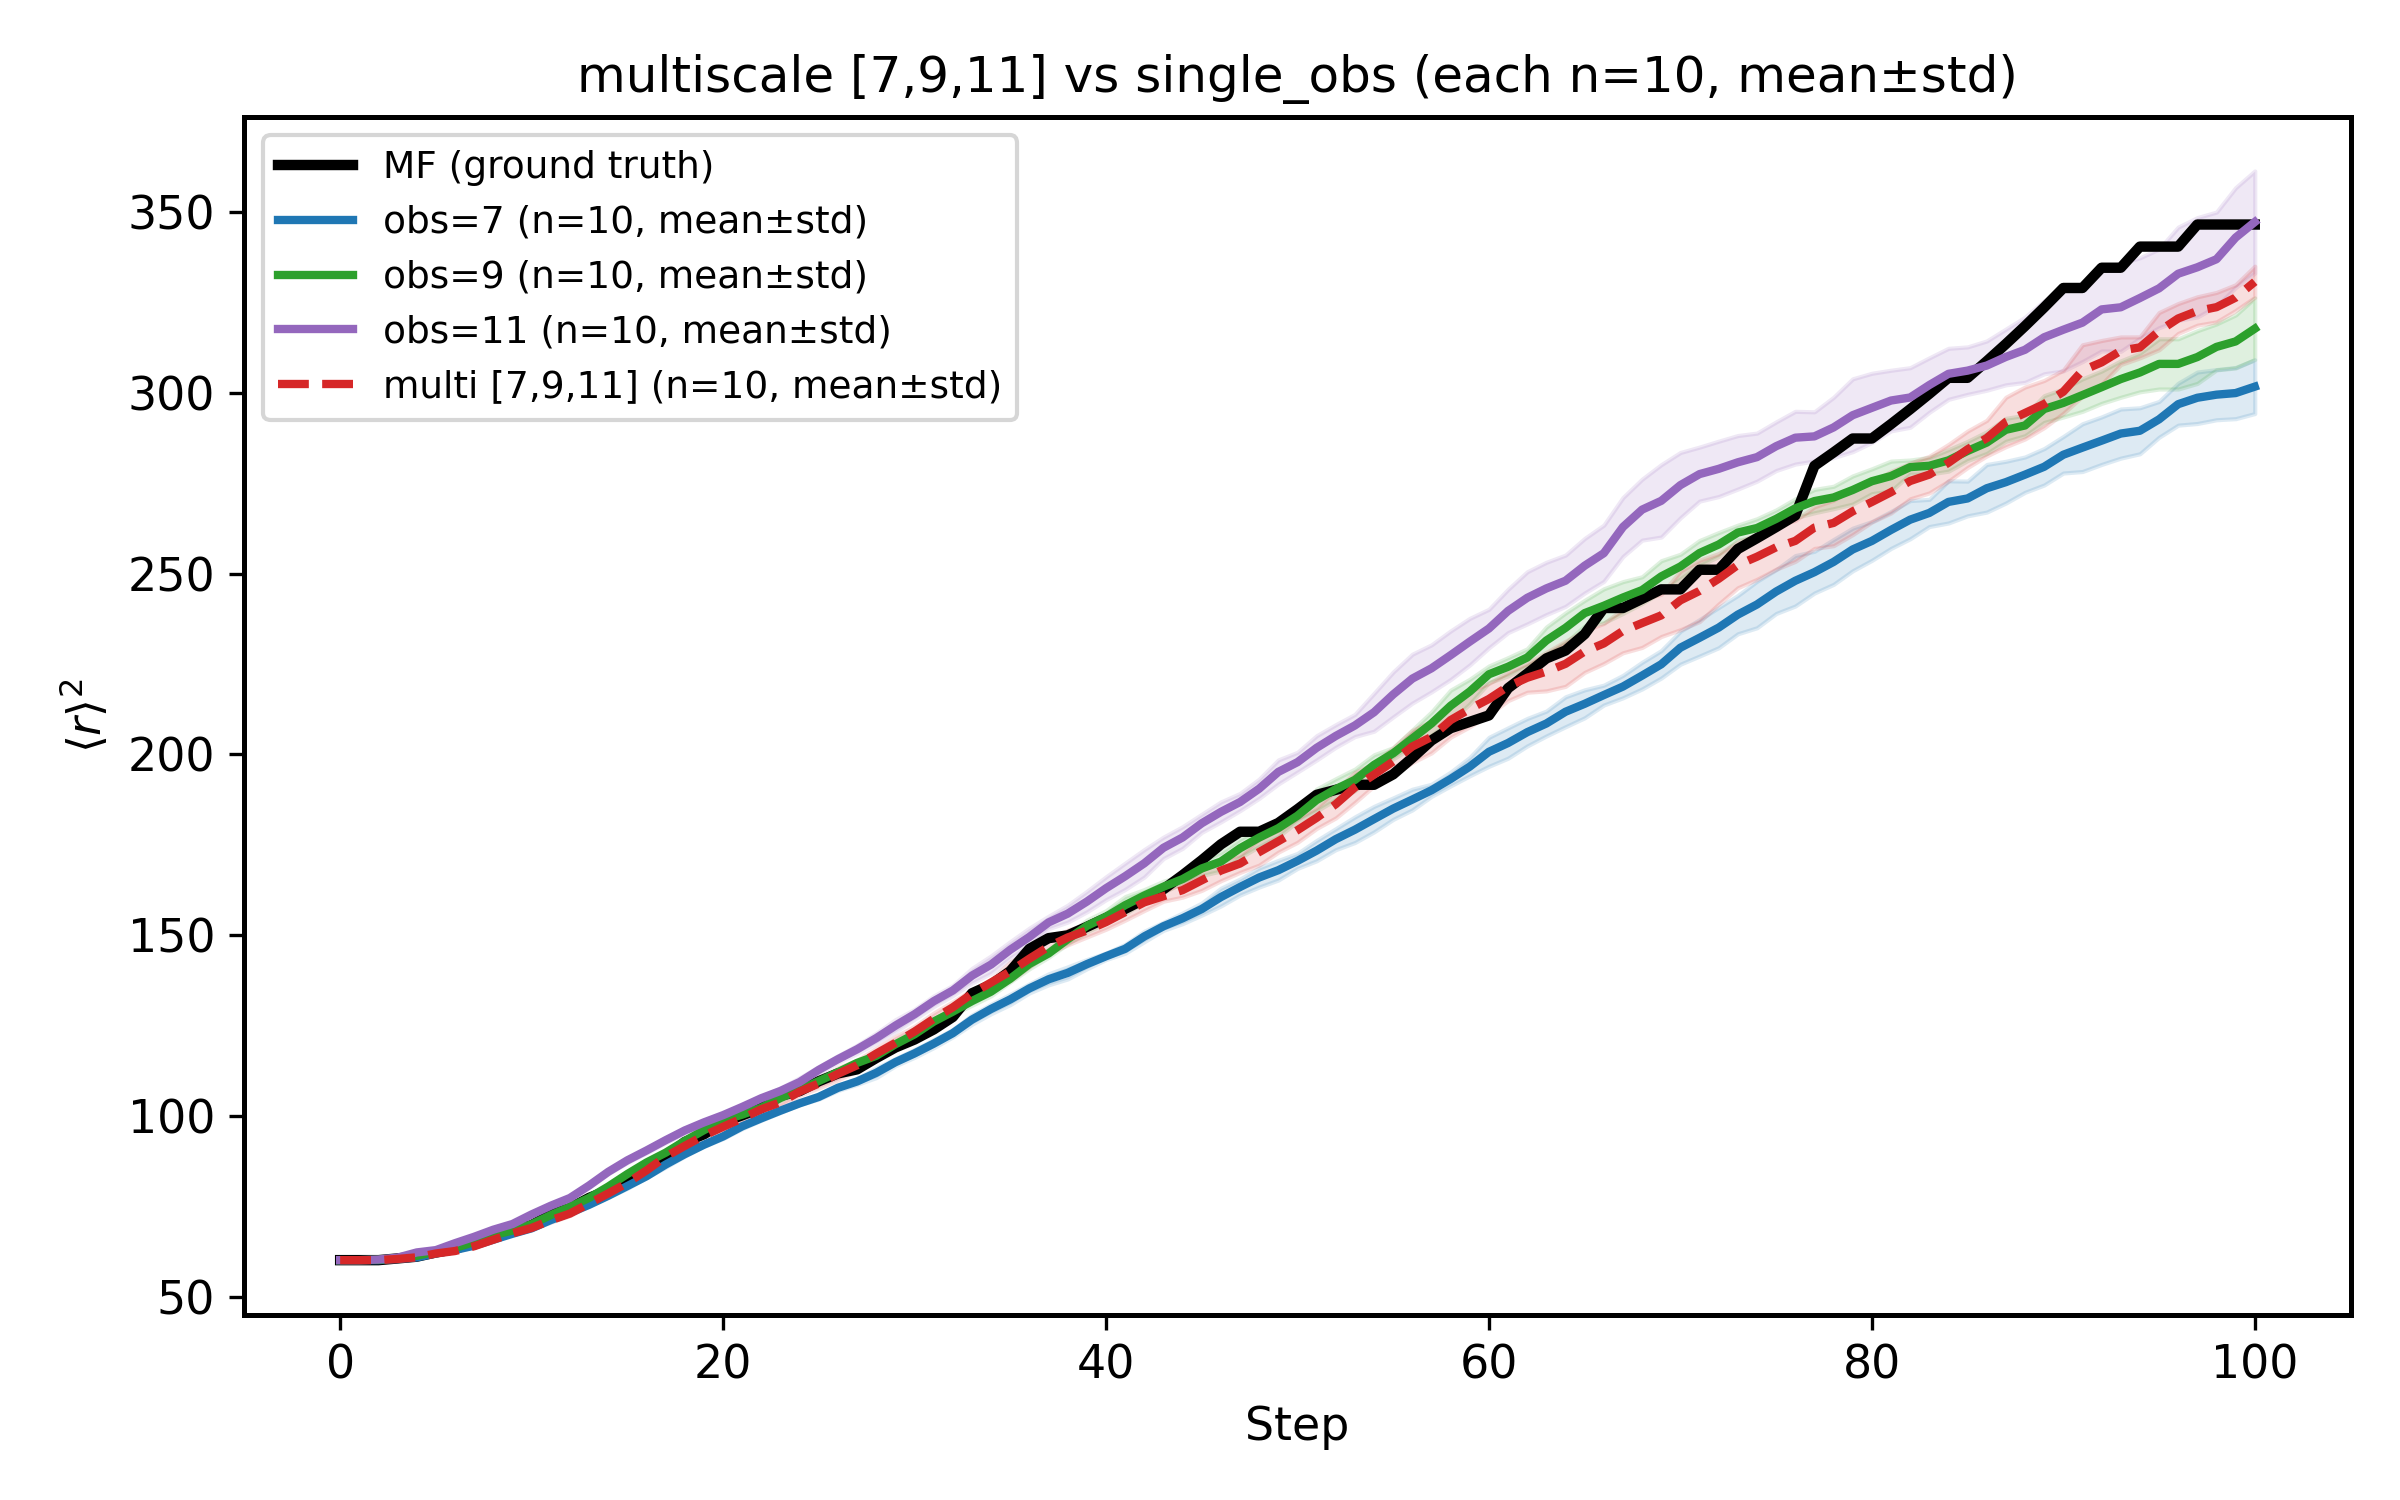
\includegraphics[alt={Mean squared radius trajectories for reference, single-scale, and multiscale model ensembles},width=0.96\textwidth]{figures/aim3_multiscale_r2_vs_step.png}

\smallskip

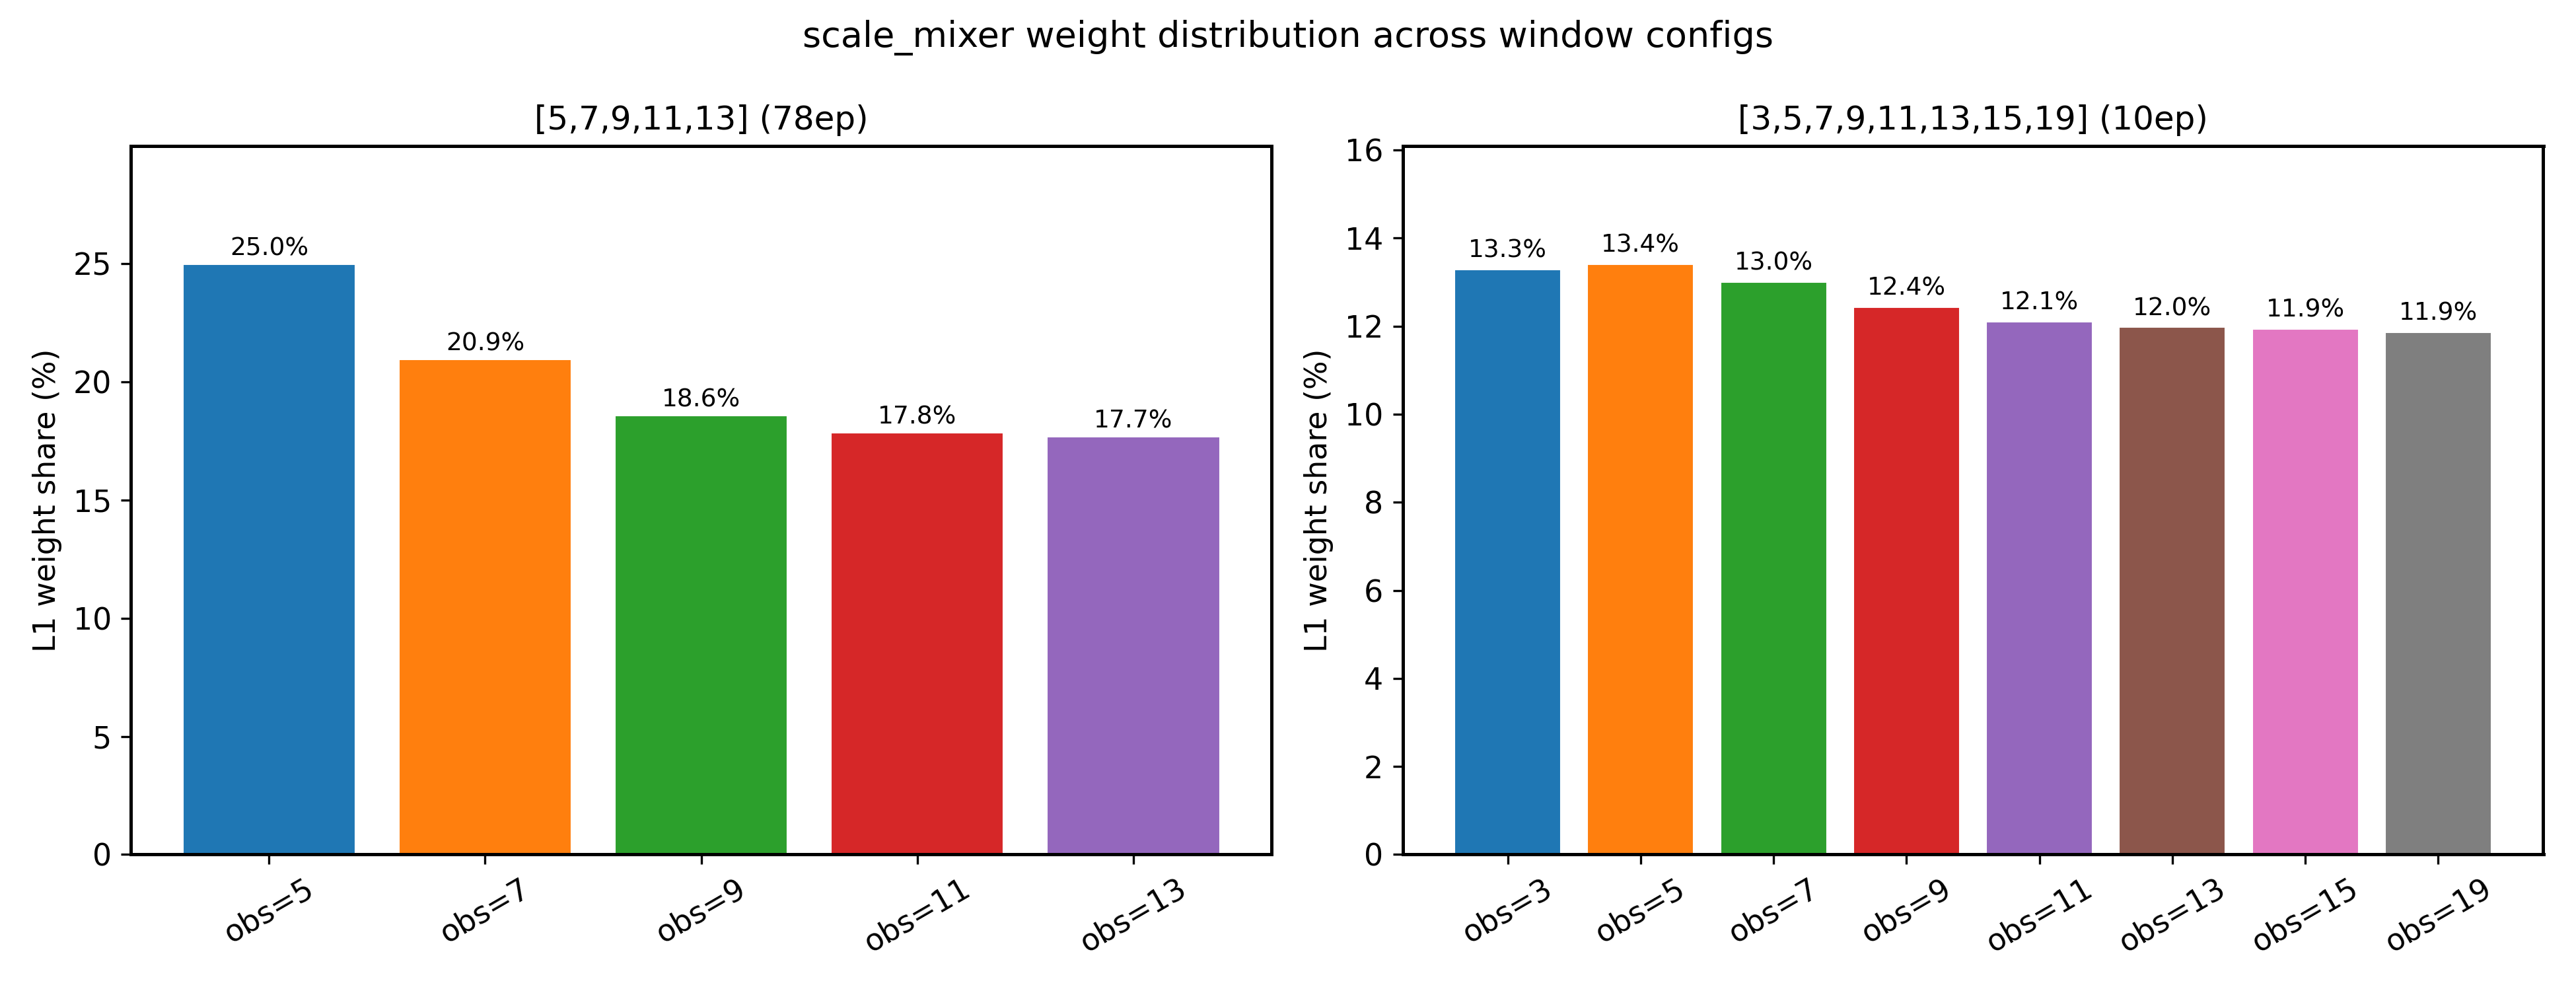
\includegraphics[alt={Relative scale-mixer weights across spatial observation windows},width=0.96\textwidth]{figures/aim3_scale_mixer_weights.png}
\caption{Existing simulation-domain results used directly for input-side interpretability. Top: \(\langle r^2\rangle\) trajectories over 100 rollout steps for the MF reference and the single- and multiscale model ensembles; bands summarize variation across ten seeds. Bottom: relative \(L_1\) scale-mixer weights for two multiscale configurations. Multiscale prediction improves trajectory fidelity, while the learned mixer places greater parameter weight on smaller observation windows. Mixer norms remain attribution indicators, not physical causal effects, until functional ablation supports them.}
\label{fig:aim3-input-prelim}
\end{figure}

\subsubsection{Output-side response probing.}
Exploratory analyses of the simulation-trained operator supply three complementary response measurements, described below: curvature-conditioned confidence, the spatial distribution of action likelihood, and full-Jacobian sensitivity.

\textbf{Curvature-conditioned confidence.} For boundary voxel \(i\), the current local curvature proxy is the number of neighboring voxels whose grain identity differs from the center in a \(3\times3\times3\) neighborhood,
\[
c_i=\sum_{j\in\mathcal{N}_{3\times3\times3}(i)\setminus i}
\mathbb{I}\!\left[g_j\neq g_i\right],
\]
where \(g_i\) is the grain identity at the center voxel. The model response is summarized by the maximum predicted transition score, \(q_i=\max_m p_i(m)\), and by output entropy. When the analysis is restricted to neighborhoods containing exactly two grain identities, \(q_i\) decreases toward the locally flat-interface proxy \(c_i\approx13\) and increases again for more strongly concave or convex configurations. Entropy shows the complementary trend. Including or excluding the center action produces no visible change because \(99.97\%\) of sampled boundary voxels select a neighboring identity. Pooling two-grain boundaries with higher-order junctions, by contrast, obscures the U-shaped response; junction neighborhoods constitute approximately \(65\%\) of the boundary-voxel population in this test. The result supports a topology-conditioned association between model confidence and a discrete curvature proxy, not direct recovery of a continuum curvature law.

\textbf{Action-field and full-Jacobian structure.} The mean \(9^3\) action-likelihood field is compact, centered to within \(0.16\) voxel, and accurately summarized by a three-dimensional Gaussian with per-voxel fitting error below \(0.01\). A full input--output Jacobian pipeline was then verified against an analytic symmetric function to machine precision. The analysis exposed a storage-axis bias introduced by the padding implementation; assigning each training sample a uniformly selected cubic-group transformation removed the systematic bias without changing validation loss. In the symmetry-controlled model, the aggregate sensitivity contains a center dip, a nearest-neighbor ring, and an approximately isotropic decay (Figures~\ref{fig:aim3-jacobian-render} and~\ref{fig:aim3-output-prelim}), while each directional output preferentially responds to the input in its own direction.

Let \(S(r)\) denote the shell mean of the voxelwise total sensitivity \(S(n)\) at distance \(r\) from the neighborhood center. This radial sensitivity is currently represented by a Shell-Gauss+\(C\) candidate model,
\[
S(r)=
A_{\mathrm{shell}}
\exp\!\left[-\frac{(r-r_0)^2}{2\sigma_{\mathrm{shell}}^2}\right]
+
A_{\mathrm{bg}}
\exp\!\left[-\frac{r^2}{2\sigma_{\mathrm{bg}}^2}\right]
+C.
\]
The fitted expression is
\[
S(r)=
0.032
\exp\!\left[-\frac{(r-0.98)^2}{2(0.67)^2}\right]
+
0.022
\exp\!\left[-\frac{r^2}{2(1.75)^2}\right]
+0.011.
\]
The first term describes a sensitivity shell centered at approximately one voxel, the second describes a broader short-range background, and \(C\) represents the nonzero long-range tail. The fit uses shell means over the radial domain while excluding the eight corner voxels at \(r\approx6.93\). Figure~\ref{fig:aim3-jacobian-render} keeps the distinction between the measured aggregate Jacobian and its radial approximation explicit: the former is computed directly from network derivatives, whereas the latter is a smooth post-hoc representation of that response. The fit is a candidate summary of the learned response, not an independently learned kernel, a finalized physical law, or proof that a unique physical mechanism has been recovered.

\begin{figure}[htbp]
\centering
\begin{minipage}[t]{0.49\textwidth}
\centering
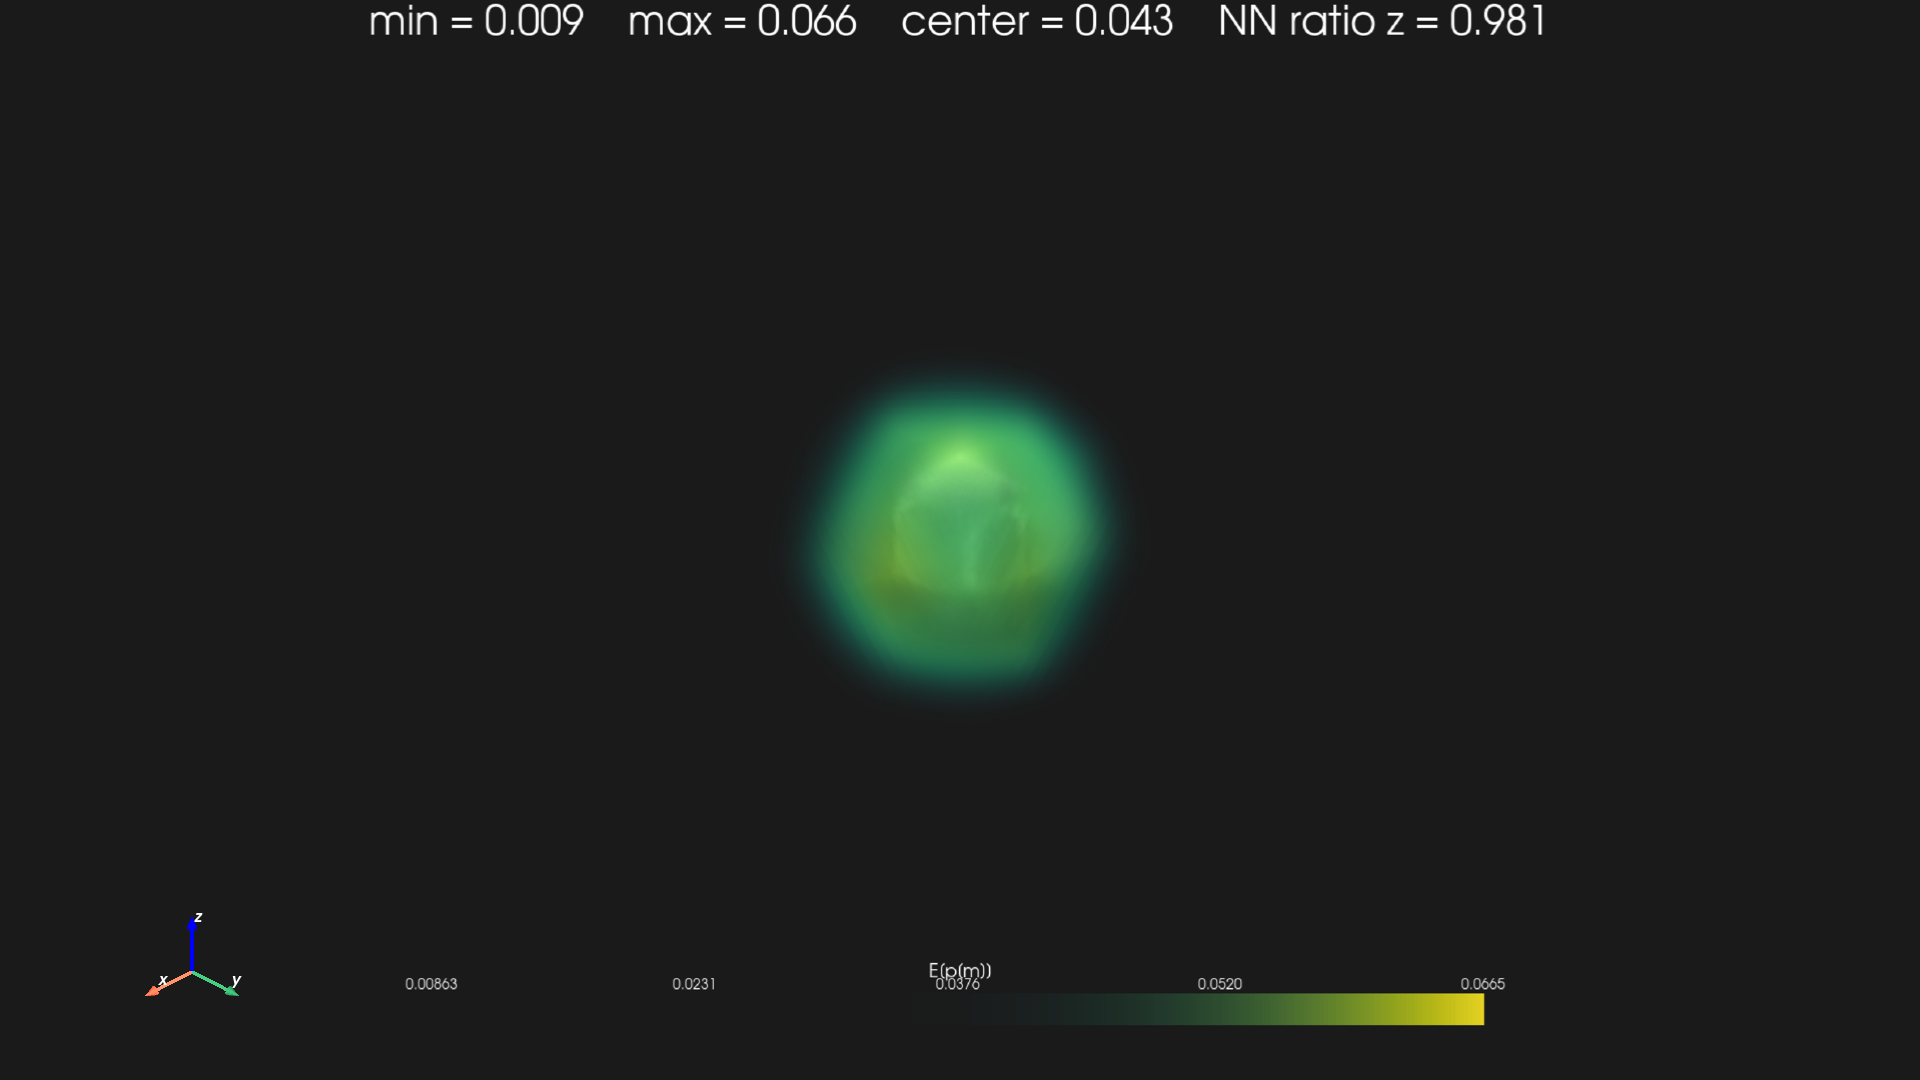
\includegraphics[alt={Three-dimensional network-derived aggregate Jacobian sensitivity},width=\linewidth,trim=250 0 250 0,clip]{figures/aim3_jacobian_actual_render.png}

\small (a) Network-derived aggregate Jacobian sensitivity
\end{minipage}
\hfill
\begin{minipage}[t]{0.49\textwidth}
\centering
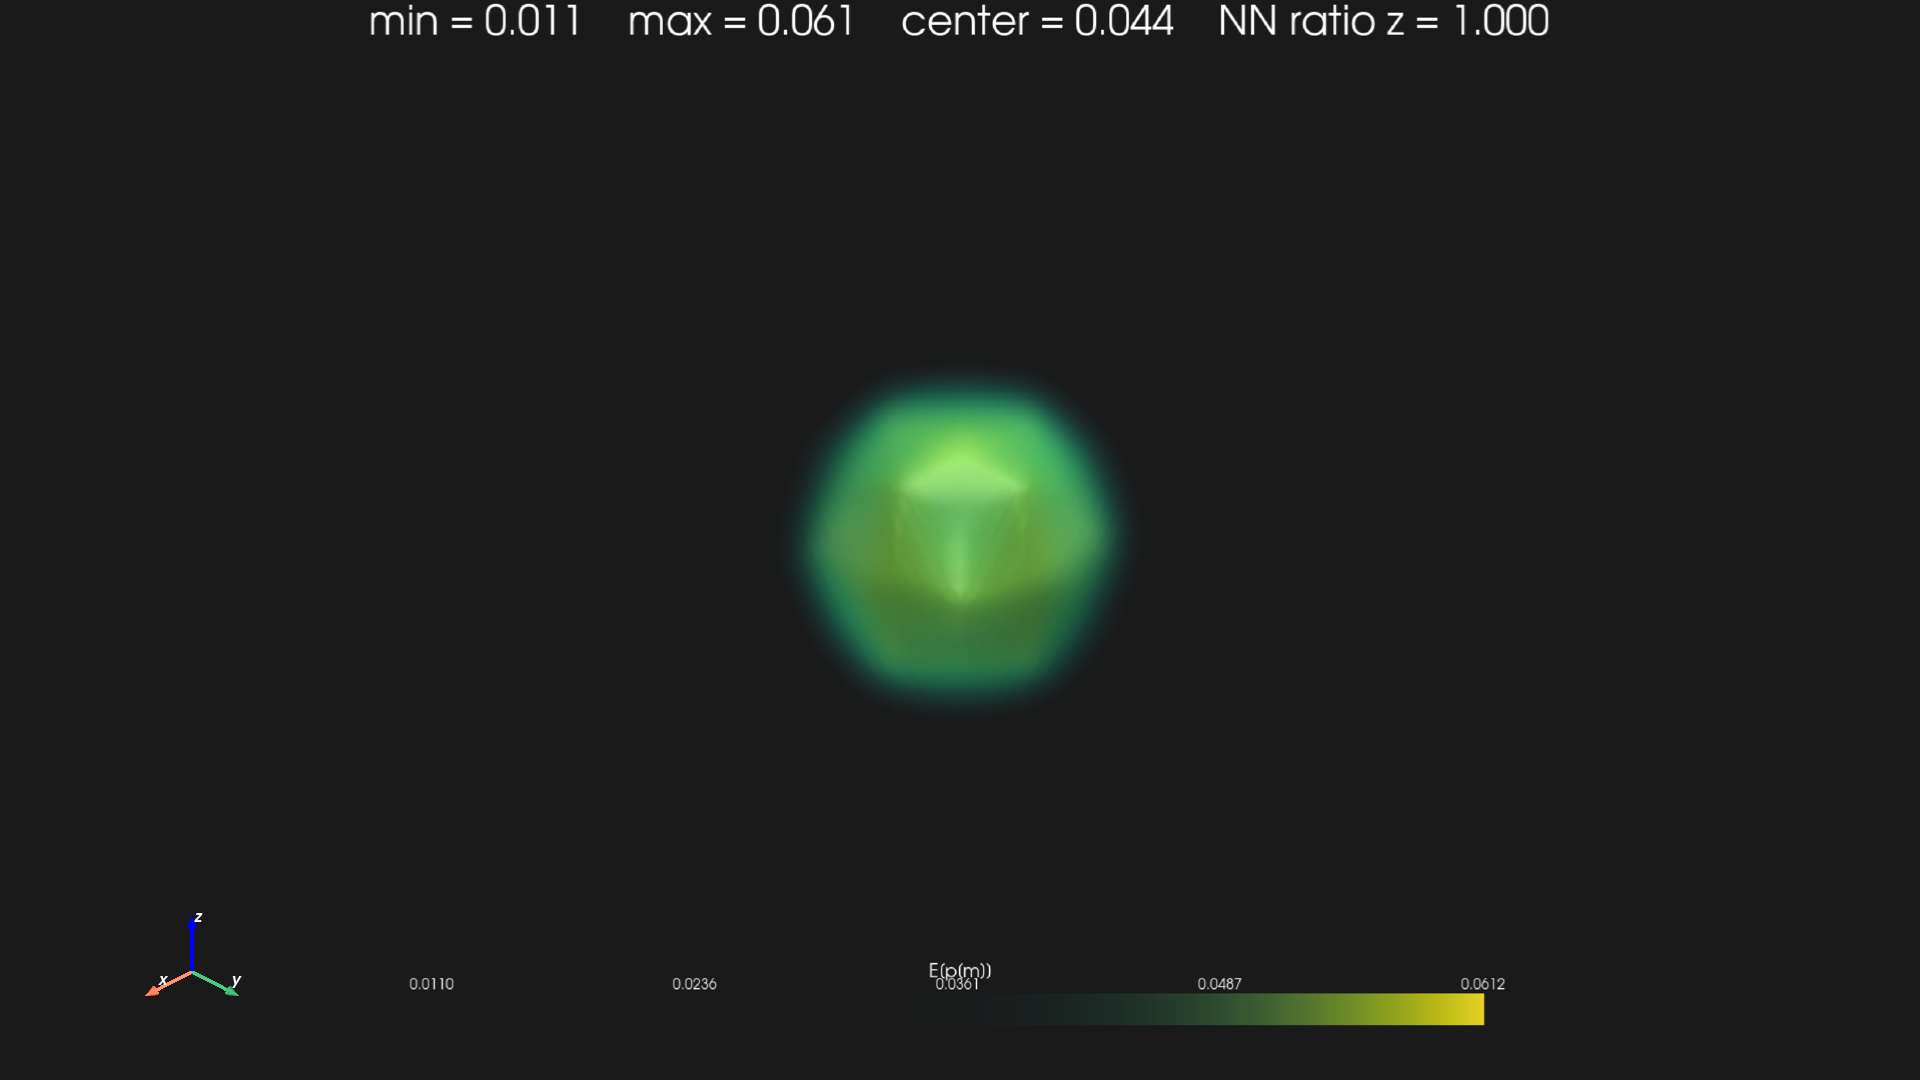
\includegraphics[alt={Three-dimensional radial Shell-Gauss plus constant approximation of Jacobian sensitivity},width=\linewidth,trim=250 0 250 0,clip]{figures/aim3_jacobian_shellgauss_c_render.png}

\small (b) Radial Shell-Gauss+\(C\) approximation
\end{minipage}
\caption{Three-dimensional comparison of the learned operator's output-side response and its compact radial approximation. (a) The aggregate sensitivity is computed directly from the mean absolute full Jacobian and summed over all 729 output positions; it retains voxel-scale deviations from perfect radial symmetry. (b) The Shell-Gauss+\(C\) function is fitted to radial shell means and evaluated on the same \(9^3\) grid; it enforces a smooth isotropic response while preserving the nearest-neighbor shell, broader short-range component, and nonzero tail. The right panel is a post-hoc summary of the left panel, not a second independently learned kernel.}
\label{fig:aim3-jacobian-render}
\end{figure}

\begin{figure}[htbp]
\centering
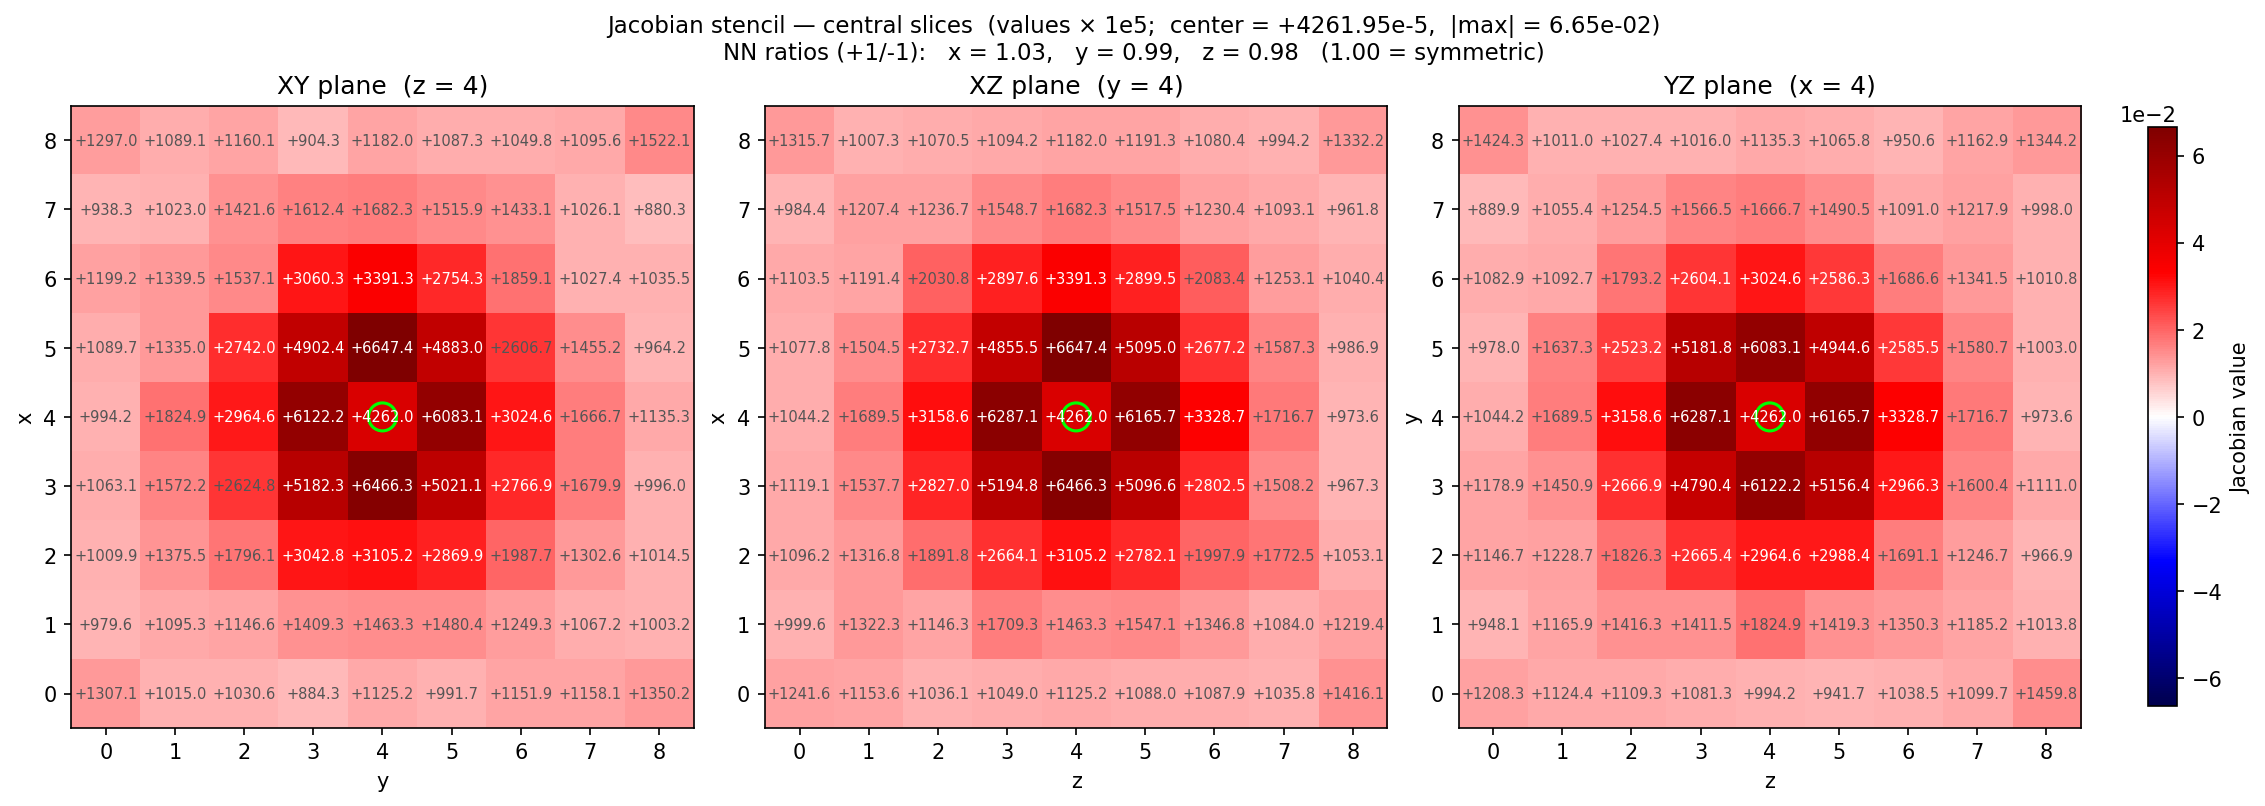
\includegraphics[alt={Orthogonal central slices through total absolute input sensitivity},width=0.98\textwidth]{figures/aim3_total_input_sensitivity_slices.png}

\smallskip

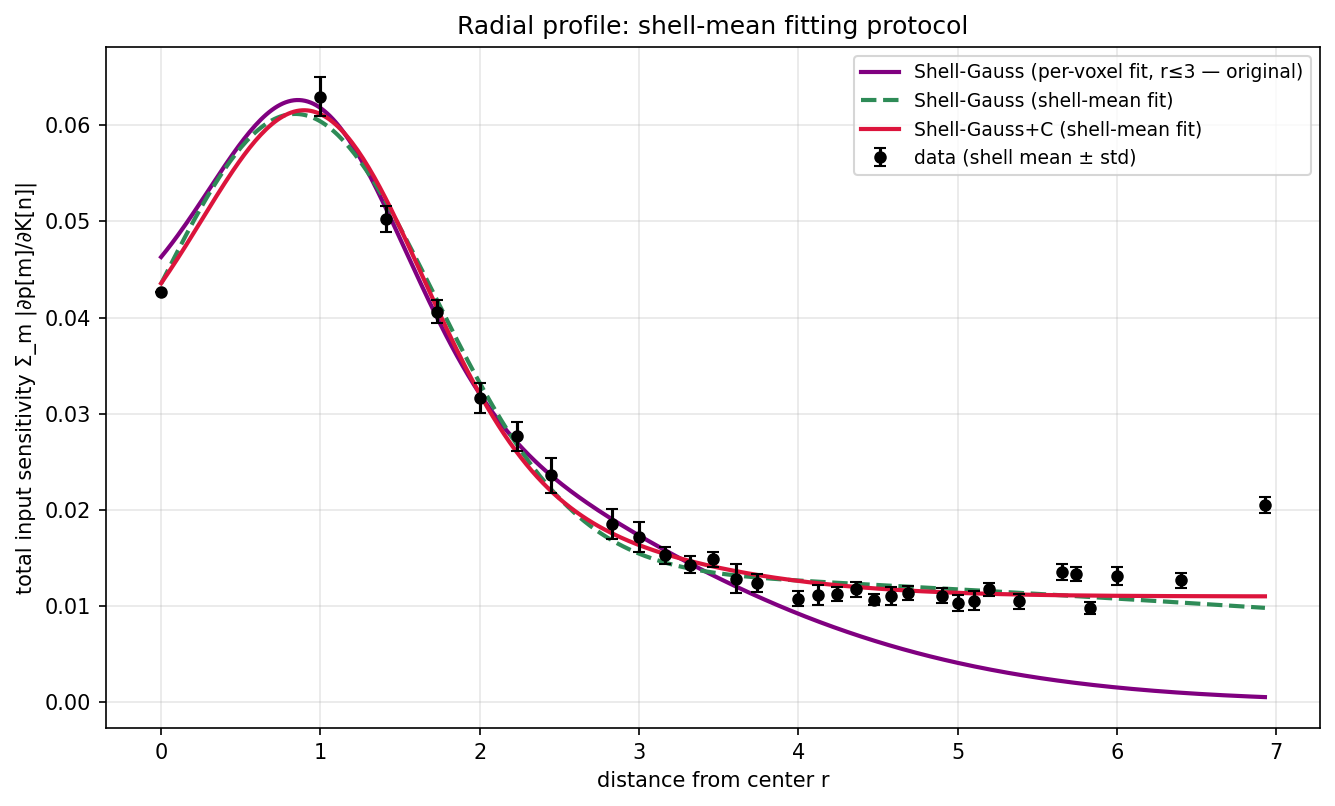
\includegraphics[alt={Shell-averaged radial sensitivity and three candidate response fits},width=0.90\textwidth]{figures/aim3_jacobian_radial_fit.png}
\caption{Existing full-Jacobian results used directly for output-side response probing. Top: three orthogonal central slices of the total absolute input sensitivity for the cubic-group-symmetrized all-voxel model. The sensitivity is approximately axis symmetric and contains a center dip surrounded by a stronger nearest-neighbor response. Bottom: shell-averaged radial sensitivity and three candidate fits, showing a nearest-neighbor-scale maximum followed by short-range decay and a nonzero tail. The fitting comparison remains exploratory; no functional form is treated as a finalized physical law.}
\label{fig:aim3-output-prelim}
\end{figure}

\subsection{Proposed methodology}

\subsubsection{Aim 3A: Determine which spatial scales drive reliable experimental predictions.}
For experiment-trained models retained after Aim 1, matched single-scale and multiscale configurations will be evaluated using the experimental Level 1--2 criteria established there. Comparing or transferring scale conclusions across simulation- and experiment-trained models lies outside the core plan, since the two sources do not yet share an audited set of commensurate metrics. If \(W_s\) denotes the block of the scale-mixing layer associated with observation scale \(s\), its global parameter-based importance will be summarized as
\[
I_s=\frac{\lVert W_s\rVert_1}{\sum_{r\in\mathcal{S}}\lVert W_r\rVert_1}.
\]
Because parameter magnitude is not equivalent to functional importance, \(I_s\) will be tested against scale removal, scale masking, and matched single-scale performance. Scale rankings and ablation effects will be estimated across model initializations and across the experimental windows that satisfy the Aim 1 reliability criteria. Prediction-horizon perturbations will test whether longer temporal targets increase dependence on broader spatial context.

\subsubsection{Aim 3B: Map how local information is converted into evolution decisions.}
Let \(K_i(n)\) denote input feature \(n\) in local sample \(i\), and let \(p_i(m)\) denote the predicted transition score for output position \(m\). The full input--output Jacobian is
\[
J_i(m,n)=\frac{\partial p_i(m)}{\partial K_i(n)}.
\]
The ensemble absolute sensitivity and total sensitivity of input position \(n\) will be calculated as
\[
\overline{J}_{\mathrm{abs}}(m,n)=\frac{1}{N}\sum_{i=1}^{N}\left|J_i(m,n)\right|,
\qquad
S(n)=\sum_m\overline{J}_{\mathrm{abs}}(m,n).
\]
Signed means will be reported together with absolute sensitivity and the sign-agreement ratio
\[
R(m,n)=
\frac{\left|\sum_i J_i(m,n)\right|}
{\sum_i\left|J_i(m,n)\right|},
\]
so that cancellation is not mistaken for weak dependence. These maps will quantify the spatial range, symmetry, and directional routing of the learned response. They will be complemented by action-likelihood maps and by confidence or entropy conditioned on curvature proxy, boundary topology, and, where measurable, boundary inclination. Two-grain boundaries and higher-order junctions will be analyzed separately.

\subsubsection{Aim 3C: Distinguish model response from physical attribution.}
The interpretation pipeline will first be reproduced on simulation-trained models, where isotropy and prescribed anisotropy provide controlled tests. Cubic rotations and reflections, axis permutations, padding controls, and model replicates will be used to identify implementation-induced asymmetry before experimental results are interpreted. The same summaries will then be applied to reliable experiment-trained models. A response will advance from Level 3 model interpretation to Level 4 physical attribution only if it is reproducible across eligible experimental windows and model replicates, is associated with a measurable microstructural descriptor after relevant geometric stratification, and survives at least one held-out or controlled test. If topology fails the Aim 1 evidence gate, topology-conditioned patterns may be reported as model behavior but will not support a topology-related physical attribution. Because the present curvature result separates two-grain interfaces from higher-order junctions, that stratification must also remain stable to the Aim 1 readout, speckle, small-grain, and connectivity tests; otherwise, both the stratified curvature--confidence relationship and the junction comparison will remain exploratory Level 3 behavior. A Level 5 candidate-mechanism claim will require an additional falsifiable prediction or intervention; agreement between a sensitivity map and a familiar physical pattern alone will not be sufficient.

\subsection{Required data and resources}

The work will use the existing multiscale and Jacobian simulation studies, symmetry-controlled simulation checkpoints, the reliable experiment-trained checkpoints and held-out predictions from Aims 1 and 2, and local descriptors derived from registered grain-ID volumes. Required descriptors include neighborhood composition, the current curvature proxy, boundary topology, and boundary inclination when it can be estimated at adequate spatial resolution.

\subsection{Quantitative validation criteria}

All interpretation summaries will be reported across model replicates with bootstrap or replicate-based uncertainty. Input-side conclusions must be supported by agreement between scale-mixer rankings and at least one functional ablation. Output-side conclusions must be stable to sample size, signed-versus-absolute aggregation, cubic coordinate transformations, and the eligible experimental-window partition. Physical attribution requires a consistent effect direction across reliable windows, uncertainty that excludes the prespecified null contrast, and successful replication in a held-out window or controlled simulation. These criteria correspond to Levels 3--4 of Table~\ref{tab:evidence-ladder}; Level 5 additionally requires a falsifiable prediction or intervention. Exact numerical tolerances for map similarity and descriptor effects will be frozen after the Aim 1 eligible-window set is known and before the final Aim 3 comparison.

\subsection{Expected outcome}

Aim 3 is expected to produce a scale-resolved and spatially resolved account of how reliable experiment-trained models convert local microstructure into evolution decisions. The result will identify which response signatures are stable model properties, which can be attributed to measurable interface geometry, and which remain testable candidate explanations short of established mechanisms.

\subsection{Risks}

Raw scale weights may not reflect functional importance; geometry descriptors may be correlated; experimental resolution may make local curvature or inclination estimates noisy; and subtle numerical anisotropy may be comparable to the physical signal. Interpretation may also vary across otherwise acceptable experimental windows.

\subsection{Alternative strategies}

If mixer weights are unstable, scale-removal and matched single-scale experiments will become the primary input-side evidence. If voxel-level Jacobians are too noisy, sensitivity will be aggregated by radial shell, direction, boundary class, or grain and evaluated as an ensemble quantity. If curvature and topology cannot be separated observationally, controlled simulation perturbations will define the claim ceiling. If no unique physical attribution survives the reliability tests, the aim will report validated model interpretation without escalating to a mechanism claim.

\subsection{Deliverables}

\begin{itemize}

\item a reproducible input-side scale-attribution analysis for simulation- and experiment-trained operators;

\item symmetry-audited output-response and full-Jacobian maps;

\item an evidence matrix separating model interpretation, physical attribution, and candidate mechanism testing;

\item a dissertation chapter and/or manuscript on interpretable learning of three-dimensional grain-growth evolution.

\end{itemize}

\bigskip

\section{Dependency and integration across aims}

The dependency chain is what makes an unfavorable result usable. Each aim inherits the evidence gate of the one before it, so a failure narrows the domain of the claim instead of ending the program:

\begin{itemize}

\item If Aim 1 finds that performance depends strongly on one window or overlap block, the valid domain will be narrowed and broader spatial-reproducibility claims will be withheld.

\item If a metric family fails the Aim 2 training-blind test, that experimental model output will not be interpreted physically, however well the same family is reproduced in the simulation domain.

\item If a family passes but does not separate from its frozen null, it will be recorded as uninformative, not as evidence of predictive fidelity.

\item If every family passes, the result establishes validated fidelity within the evaluated experimental domain but does not by itself prove that the operator has recovered material physics absent from the simulator.

\item If Aim 3 supports stable model interpretation but not unique physical attribution, the dissertation will stop at the appropriate evidentiary level.

\end{itemize}

One local architecture, data representation, rollout code, replicate policy, and evidence ladder serve all three stages; what changes is the supervision source and the strength of claim the validation permits. Aim 3 implementation and diagnostic development may overlap with Aim 2 in time, but final experimental interpretation will be restricted to outputs that are both Aim 1 eligible and Aim 2 validated.


\chapter{Expected Outcomes, Contributions, and Scientific Impact}

\section{Established foundation}

The completed work establishes two linked results: local neighborhood design controls the effective inclination response encoded by stochastic simulation labels, and a fixed local three-dimensional operator can learn and scale those controlled rules. These results supply the physical and computational foundation for the proposed transition to experimental supervision; they are not repeated here as future deliverables.

\section{Guaranteed analytical and methodological contributions}

The following contributions are guaranteed in the sense that they are completed analyses or prespecified deliverables, not guaranteed favorable outcomes:

\begin{itemize}
\item a reproducible, label-preserving workflow for converting sparse 4D categorical grain maps into local supervision, including quantitative registration, linkage, drift, and retained-volume diagnostics;
\item a geometric and data-quality assessment of the experimental volume's support for spatial validation; if too few sufficiently separated windows survive curation, the result will become a quantitative bound on within-volume spatial reproducibility instead of an unsupported independence claim;
\item prespecified persistence, majority-class, distributional, readout, and topology-sensitivity baselines;
\item a frozen, training-blind validation protocol for experiment-trained rollout that keeps fidelity to the simulation teacher distinct from fidelity to experiment and records failed metrics instead of averaging them away;
\item symmetry-audited multiscale and Jacobian interpretation methods transferred to the strongest experiment-trained models supported by Aims 1--2;
\item an explicit domain-of-applicability and evidence-level statement, even if that domain is narrow.
\end{itemize}

These outputs shift the central methodological question from whether a network can fit one favorable transition to which evidence is required before a measured or simulated rollout can be used scientifically.

\section{Conditional scientific contributions}

Broader claims remain conditional on the achieved evidence. If uncertainty indicators track held-out failure, Aim 1 may support a practical abstention rule. If the training-blind evaluation separates from its frozen null baselines, Aim 2 may establish a validated domain of applicability for the experiment-trained operator. If Aim 3 responses reproduce across eligible windows, model initializations, geometric strata, and controlled tests, selected signatures may advance from stable model interpretation to physical attribution. Formal probabilistic calibration, broad transfer, and a unique mechanism claim are not guaranteed.

\section{Scientific impact}

For experimental materials science, the work provides a way to use sparse 4D grain maps without allowing registration or segmentation structure to masquerade as dynamics. For mesoscale modeling, it separates control of the simulation teacher from fidelity of its surrogate and from fidelity to experiment. For scientific machine learning, it demonstrates a reusable evidence ladder linking field integrity, mesoscale prediction, model interpretation, and physical attribution. A curated dataset or software release would further broaden this impact, but public release will be promised only after data ownership and sharing permissions are confirmed.


\chapter{Research Timeline and Dissertation Plan}

\section{Research timeline and scope control}

The schedule is planned backward from the May 2027 completion target. Research and writing overlap so that the dissertation is not postponed until all analysis is complete.

To protect the core scope, the schedule prioritizes Aim 1 window-feasibility and spatial-reproducibility analysis, preserves the Aim 2 training-blind validation, and bases final Aim 3 claims on validated outputs. External datasets, new materials, a direct MF rollout initialized from an experimental state, broad architecture sweeps, and full probabilistic calibration remain outside the core plan.

One further analysis is deferred to the same category. The simulation and experimental fidelity profiles are kept separate throughout this proposal, and no nominally shared metric is assumed to mean the same thing in both. Auditing that assumption, by applying experimental observation operators such as resolved-grain cutoffs, connectivity rules, and identity censoring to simulation trajectories and asking which metrics survive as commensurate, is a coherent study in its own right. It contributes nothing to the Aim 2 validation claim, and it will be attempted only if the three aims finish with time remaining.

\begin{table}[htbp]
\centering
\caption{Proposed research, writing, and decision timeline toward the May 2027 completion target.}
\label{tab:research-timeline}
\small

\begin{tabularx}{\textwidth}{@{}*{4}{>{\raggedright\arraybackslash}X}@{}}

\toprule

\textbf{Period} & \textbf{Primary research activity} & \textbf{Writing and deliverable} & \textbf{Decision point} \\

\midrule

August-September 2026 & Quantify window geometry, overlap, quality, and effective independence; complete curation, registration, and linkage & Draft introduction, competitive positioning, and completed foundations & Which blocked spatial design is supported by the admissible windows? \\

October-November 2026 & Train and evaluate grouped-window replicate models; calculate null/readout baselines and the reliability matrix & Draft Aim 1 methods and preliminary-results chapter & Does performance reproduce across supported partitions and outperform nulls? \\

December 2026 & Complete core empirical uncertainty and domain-of-applicability analysis & Finalize Aim 1 figures, tables, and chapter & Which outputs are reliable enough for Aim 2 and interpretation? \\

January-February 2027 & Freeze the Aim 2 evaluation protocol, tolerances, and evaluated partition; complete model selection using Aim 1 material only & Draft Aim 2 methods and validation-protocol section & Is the protocol complete enough to freeze before unblinding? \\

March 2027 & Execute the training-blind evaluation; compute null comparisons, replicate spread, uncertainty, and failure modes & Finalize Aim 2 figures, validation matrix, and chapter & Which metric families pass, partially pass, or fail? \\

February-April 2027, overlapping & Begin provisional Aim 3 implementation, then restrict final analyses to outputs that are both Aim 1 eligible and Aim 2 validated & Complete Aim 3 figures, evidence matrix, and synthesis & Which signatures support Level 3 interpretation, Level 4 attribution, or Level 5 testing? \\

April 2027 & Integrate aims, limitations, contributions, and conclusions & Full revision and committee feedback & Are all claims consistent with achieved evidence? \\

May 2027 & Complete final analyses, formatting, submission, and defense preparation & Final dissertation and manuscript package & Completion \\

\bottomrule
\end{tabularx}
\end{table}

\bigskip

\section{Expected dissertation chapters}

The dissertation will use a seven-chapter structure that follows the causal program while avoiding unnecessary separation of the current experimental manuscript from its multi-window extension.

\begin{table}[htbp]
\centering
\caption{Provisional dissertation chapter structure, scientific role, and current maturity.}
\label{tab:dissertation-chapters}
\small

\begin{tabularx}{\textwidth}{@{}*{4}{>{\raggedright\arraybackslash}X}@{}}

\toprule

\textbf{Chapter} & \textbf{Working title} & \textbf{Role} & \textbf{Maturity} \\

\midrule

1 & Introduction: Learning Grain-Growth Dynamics Across Simulation and Experiment & Overarching question, background, and source-aware framework & To be written \\

2 & Neighborhood-Driven Anisotropy and Lattice Pinning in Stochastic Grain-Growth Models & Establish physical control of simulation labels & Completed prior work \\

3 & A Physics-Regulated Neural Framework for Learning 3D Grain-Growth Dynamics & Establish scalable learning of controlled simulation rules & Completed prior work; under review \\

4 & Experimentally Grounded Learning: Curation, Direct Training, and Spatial Reproducibility & Stable preliminary evidence and Aim 1 & Ongoing/proposed \\

5 & Training-Blind System Validation of Experiment-Trained Rollout & Aim 2 frozen protocol, null comparisons, and validation matrix & Proposed \\

6 & Interpretability and Physics Learning from Experimentally Learned Evolution Rules & Aim 3 & Probe development completed; experimental application proposed \\

7 & Integrated Conclusions and Future Directions & Cross-aim synthesis, limitations, and broader implications & To be written \\

\bottomrule
\end{tabularx}
\end{table}

Each chapter will state the assumption it controls or removes, the evidence it contributes to the central hypothesis, and the limitation that motivates the next chapter. Shared notation, maturity labels, and validation metrics will prevent the dissertation from reading as three disconnected papers.


\chapter{Conclusion}

Four things have to hold before a learned grain-growth operator can be trusted: control of the label source, field-level integrity checks, mesoscale validation against the correct reference, and evidence gates between prediction and interpretation. The completed neighborhood and 3D-PRIMME studies establish the simulation foundation. The experimental preliminary work demonstrates feasibility while exposing the limits that remain in space, time, topology, and measurement.

The proposed work will quantify spatial reproducibility within the available volume, establish null and artifact-sensitive baselines, and then apply those frozen definitions once to an experimental partition used for neither training nor model selection. Only outputs that survive that test will undergo multiscale and Jacobian interpretation. The resulting contribution is a source-aware framework that reports what a local operator predicts together with the evidence that supports using or interpreting the prediction.


\clearpage
\section*{Open Questions for the Committee}
\addcontentsline{toc}{chapter}{OPEN QUESTIONS FOR THE COMMITTEE}

Several decisions are deliberately left open until the underlying measurement is in hand, since fixing them now would amount to choosing a threshold before knowing what the data support. Committee guidance is welcome on each.

\begin{enumerate}

\item \textbf{Window admissibility.} The candidate-window stride, overlap graph, and quality distribution will determine how many windows survive curation, and therefore what spatial design Aim 1 can support. Is a within-volume reproducibility result acceptable if only three or four windows qualify?

\item \textbf{Aim 1 thresholds.} Partition design, replicate budget, and prospective pass/fail thresholds will be fixed once the admissible-window count is known. \texttt{[NEEDS QUANTITATIVE CRITERION]}

\item \textbf{Aim 2 freeze.} The evaluated partition, per-family tolerances, uncertainty estimator, effective-time policy, and the protocol-freeze date all need to be recorded before unblinding. \texttt{[NEEDS QUANTITATIVE CRITERION]}

\item \textbf{Aim 3 escalation.} What evidence would the committee require before a reproducible response signature is reported as physical attribution rather than model behavior?

\item \textbf{Data release.} DCT data ownership, the availability of another specimen or time state, and permission to release curated data or code remain to be confirmed.

\item \textbf{Scope of the single dataset.} The plan assumes one five-state volume. If the committee regards a second specimen as necessary for the dissertation, that decision is best made now rather than after Aim 1.

\end{enumerate}


\end{document}
